\documentclass[a4paper,12pt]{article}



% Pacotes essenciais
\usepackage[brazil]{babel}
\usepackage[T1]{fontenc}

% Pacotes para citações no estilo ABNT
\usepackage[alf]{abntex2cite}

% Pacotes adicionais
\usepackage{csquotes, graphicx, xcolor, comment, enumerate, multirow, 
    multicol, titlesec, amsmath, amsthm, amsfonts, amssymb, dsfont, 
    blindtext, ragged2e, array, enumitem, tikz, bbding, pifont, wasysym, 
    titling, longtable, fancyhdr, url, float, placeins, xurl}

\usepackage{graphicx}\usepackage[table]{xcolor}
% Configuração de margens
\usepackage[lmargin=2cm, rmargin=2cm, tmargin=2cm, bmargin=2.5cm]{geometry}

% Configuração do cabeçalho com logo
\usepackage{fancyhdr}
\pagestyle{fancy}
\fancyhf{}
\renewcommand{\headrulewidth}{0pt} % Remove a linha no cabeçalho
\rhead{\transparent
\includegraphics[width=2cm]{./assets/logocogel.jpg}} % Certifique-se do caminho correto

% Configuração do hyperref (deve ser o último pacote)
\usepackage{hyperref}
\hypersetup{
    colorlinks=true,
    linkcolor=blue, % Cor dos links internos (tabelas, figuras, etc)
    urlcolor=blue,  % Cor dos links externos
    citecolor=green % Cor das citações
}

\usepackage{helvet}
\renewcommand{\familydefault}{\sfdefault}

% Configuração da bibliografia (ABNT)
\bibliographystyle{abntex2-alf}
 
\title{Relatório de Auditoria de Segurança Cibernética}
\author{}
\date{}
\begin{document}


\begin{center}
    \large{\textbf{Companhia de Governança Eletrônica do Salvador\\
Diretoria Técnica e de Infraestrutura\\
Gerência Especial de Segurança da Informação\\
}}

\vspace{7cm}

\Large{Relatório de Auditoria de Segurança Cibernética\\
teste - teste}

\vspace{4cm}
\textcolor{red}{CONFIDENCIAL}
\end{center}
\newpage

\tableofcontents  %Sumario


\newpage

\section{Introdução}
\subsection{Objetivo}
Este relatório, elaborado pela \textbf{Gerência Especial de Segurança da Informação da COGEL}, apresenta os resultados da auditoria de segurança cibernética realizada no ambiente de aplicações e servidores da Prefeitura de Salvador, administrado pela empresa teste - teste. O objetivo principal é identificar vulnerabilidades e riscos associados à segurança da informação, avaliar a conformidade com as normas e padrões de segurança aplicáveis, e fornecer uma visão abrangente do estado atual da segurança cibernética no ambiente auditado.

\subsection{Escopo}
A auditoria abrange a avaliação das vulnerabilidades em sistemas operacionais e aplicações web, identificadas no período de 15 de janeiro de 2002 a junho.

\section{Metodologia}
\subsection{Ferramentas Utilizadas}
\begin{itemize}
    \item \textbf{Tenable.io Vulnerability Management (Nessus, NNM):} Esta ferramenta avançada de gerenciamento de vulnerabilidades permite a realização de escaneamentos automatizados para identificar falhas de segurança em sistemas e redes. Utiliza diversas técnicas de varredura para detectar vulnerabilidades conhecidas e potenciais, ajudando a priorizar a correção com base em riscos específicos.
    \item \textbf{Trend Micro XDR Vision One:} Plataforma de Detecção e Resposta Estendida (XDR) que oferece visibilidade abrangente e correlação de ameaças em múltiplos vetores, incluindo endpoints, servidores e redes. A ferramenta melhora significativamente a capacidade de resposta a incidentes, correlacionando dados de diferentes fontes para identificar atividades maliciosas de forma mais eficaz.
    \item \textbf{Microsoft Windows:} Sistema operacional desenvolvido pela Microsoft, amplamente utilizado em ambientes corporativos e pessoais. Conhecido por sua interface amigável e vasta gama de aplicações empresariais, o Windows também incorpora diversas ferramentas de segurança e gerenciamento, como o Windows Defender e o Active Directory.
    \item \textbf{Linux:} Sistema operacional de código aberto amplamente utilizado em servidores e desktops. Reconhecido por sua robustez, segurança e flexibilidade, o Linux suporta uma vasta gama de distribuições que podem ser otimizadas para diferentes propósitos, desde servidores de alta performance até dispositivos embarcados.
\end{itemize}

\subsection{Procedimentos}
A auditoria foi conduzida por meio de uma série de escaneamentos automatizados, inspeções manuais e validações de conformidade com as normas e padrões de segurança aplicáveis.

\section{Sumário Executivo}
A auditoria revelou um total de \textbf{811} ativas, distribuídas entre críticas, altas, médias e baixas. A seguir, apresentamos um resumo das principais descobertas.

\section{Análise de Vulnerabilidades e Riscos Associados}
As vulnerabilidades identificadas apresentam um risco significativo para a segurança do ambiente de TI da Prefeitura de Salvador. A seguir, destacamos os principais riscos associados a essas vulnerabilidades:

O escaneamento de vulnerabilidades dos hosts levantou um total de \textbf{17} vulnerabilidades, classificadas em críticas, altas, médias e baixas.

   \begin{figure}[h!]
    \centering
    \includegraphics[width=0.4\textwidth]{assets/images-vmscan/Total_Vulnerabilidades.png} 
    \end{figure}
    \FloatBarrier

A seguir, destacamos os principais riscos associados a essas vulnerabilidades: 

%-------------- INÍCIO DA CATEGORIA Vulnerabilidades Relacionadas à Versões não suportadas --------------
\subsection{Vulnerabilidades Relacionadas à Versões não suportadas}
Riscos provenientes do uso de software ou sistemas operacionais desatualizados e fora de suporte, que não recebem mais atualizações de segurança e permanecem vulneráveis a ataques.

%-------------- INÍCIO DA SUBCATEGORIA Protocolos e Cifras Depreciadas --------------
\subsubsection{Protocolos e Cifras Depreciadas}
Descrição não disponível.

\begin{enumerate}
%-------------- INÍCIO DA VULNERABILIDADE SSL Medium Strength Cipher Suites Supported (SWEET32) --------------
\item \textbf{\texttt{SSL Medium Strength Cipher Suites Supported (SWEET32)}}
\textbf{Descrição:} O host remoto suporta o uso de cifras SSL com força de criptografia média[cite: 151]. Cifras de força média incluem aquelas que utilizam comprimentos de chave de pelo menos 64 bits e menos de 112 bits ou aquelas que utilizam o conjunto de cifras 3DES (Triple Data Encryption Standard)[cite: 152]. A vulnerabilidade conhecida como SWEET32 explora fraquezas em cifras baseadas em 3DES devido ao seu tamanho de bloco reduzido (64 bits)[cite: 153]. Essa característica facilita ataques que dependem da repetição de blocos de criptografia (birthday attacks), especialmente em ambientes onde um grande volume de dados é transmitido pela mesma sessão criptografada[cite: 154]. A criptografia de força média é significativamente mais fácil de ser comprometida, especialmente quando o atacante está na mesma rede física do alvo[cite: 155]. O suporte a cifras de força média pode resultar em ataques de descriptografia[cite: 156], comprometimento da privacidade [cite: 157] e não conformidade regulatória[cite: 158].

\textbf{Solução:} A solução recomendada é reconfigurar a aplicação afetada para evitar o uso de cifras de força média[cite: 159]. Isso inclui desativar o suporte ao 3DES e garantir que apenas cifras fortes, que utilizem comprimentos de chave modernos e modos de criptografia robustos, sejam habilitadas[cite: 160]. A substituição de cifras de força média por alternativas mais seguras melhora a resistência contra ataques criptográficos e garante a conformidade com os padrões de segurança cibernética mais recentes[cite: 161].

\textbf{Total de Hosts Afetados:} 2

\textbf{Hosts Afetados:}
\begin{itemize}
    \item \url{172.20.13.7}
    \item \url{172.21.39.30}
\end{itemize}

%-------------- FIM DA VULNERABILIDADE SSL Medium Strength Cipher Suites Supported (SWEET32) --------------
%-------------- INÍCIO DA VULNERABILIDADE TLS Version 1.0 Protocol Detection --------------
\item \textbf{\texttt{TLS Version 1.0 Protocol Detection}}
\textbf{Descrição:} O serviço remoto está aceitando conexões criptografadas usando TLS 1.0[cite: 144]. Embora o TLS 1.0 tenha sido uma melhoria significativa em relação ao SSL, ele ainda possui várias falhas de design criptográfico[cite: 145]. Versões mais recentes do TLS, como 1.2 e 1.3, foram projetadas para resolver essas falhas de maneira mais robusta e devem ser utilizadas sempre que possível[cite: 146]. A utilização do TLS 1.0 pode expor a comunicação a falhas de design criptográfico[cite: 147], incompatibilidade com navegadores modernos [cite: 148] e não conformidade com regulamentos de segurança como o PCI DSS[cite: 149].

\textbf{Solução:} A solução para mitigar essa vulnerabilidade é habilitar o suporte para TLS 1.2 e 1.3 e desabilitar completamente o TLS 1.0[cite: 150].

\textbf{Total de Hosts Afetados:} 2

\textbf{Hosts Afetados:}
\begin{itemize}
    \item \url{172.20.13.7}
    \item \url{172.21.39.30}
\end{itemize}

%-------------- FIM DA VULNERABILIDADE TLS Version 1.0 Protocol Detection --------------
\end{enumerate}
%-------------- FIM DA SUBCATEGORIA Protocolos e Cifras Depreciadas --------------
%-------------- FIM DA CATEGORIA Vulnerabilidades Relacionadas à Versões não suportadas --------------
%-------------- INÍCIO DA CATEGORIA Vulnerabilidades relacionadas à Cifras Não suportadas --------------
\subsection{Vulnerabilidades relacionadas à Cifras Não suportadas}
Falhas associadas ao uso de algoritmos de criptografia fracos ou desatualizados, que podem ser facilmente quebrados por atacantes, comprometendo a confidencialidade dos dados.

%-------------- INÍCIO DA SUBCATEGORIA Protocolos e Cifras Depreciadas --------------
\subsubsection{Protocolos e Cifras Depreciadas}
Descrição não disponível.

\begin{enumerate}
%-------------- INÍCIO DA VULNERABILIDADE SSL RC4 Cipher Suites Supported (Bar Mitzvah) --------------
\item \textbf{\texttt{SSL RC4 Cipher Suites Supported (Bar Mitzvah)}}
\textbf{Descrição:} O host remoto suporta o uso do algoritmo de cifra RC4 em uma ou mais suítes criptográficas[cite: 181]. O RC4 possui falhas conhecidas na geração de seu fluxo de bytes pseudoaleatório, introduzindo diversos vieses que reduzem sua aleatoriedade[cite: 182]. Se um mesmo texto em claro for criptografado repetidamente (por exemplo, cookies HTTP) e um atacante conseguir capturar um grande número de textos cifrados (dezenas de milhões), há a possibilidade de inferir o conteúdo original da comunicação[cite: 183]. Isso compromete a confidencialidade dos dados transmitidos.

\textbf{Solução:} Recomenda-se reconfigurar a aplicação afetada para evitar o uso de cifras RC4[cite: 184]. Sempre que possível, utilize TLS 1.2 com suítes criptográficas baseadas em AES-GCM, garantindo compatibilidade com navegadores e servidores web suportados[cite: 185]. Essa atualização melhora a segurança das comunicações e mitiga os riscos associados ao uso de cifras obsoletas[cite: 186].

\textbf{Total de Hosts Afetados:} 1

\textbf{Hosts Afetados:}
\begin{itemize}
    \item \url{172.21.39.30}
\end{itemize}

%-------------- FIM DA VULNERABILIDADE SSL RC4 Cipher Suites Supported (Bar Mitzvah) --------------
%-------------- INÍCIO DA VULNERABILIDADE TLS Version 1.1 Deprecated Protocol --------------
\item \textbf{\texttt{TLS Version 1.1 Deprecated Protocol}}
\textbf{Descrição:} O serviço remoto analisado aceita conexões criptografadas utilizando o protocolo TLS 1.1[cite: 87]. Este protocolo está obsoleto e não oferece suporte para conjuntos de cifras atuais e recomendados[cite: 88]. Cifras que utilizam encriptação antes da computação MAC, bem como modos de autenticação como GCM (Galois/Counter Mode), não podem ser utilizados com o TLS 1.1[cite: 89]. Desde 31 de março de 2020, endpoints que não oferecem suporte ao TLS 1.2 ou superior não funcionam adequadamente com os principais navegadores da web e fornecedores de tecnologia[cite: 90]. O uso contínuo do TLS 1.1 representa um risco à segurança e à compatibilidade[cite: 91]. O suporte ao TLS 1.1 pode levar a comprometimento da segurança[cite: 92], incompatibilidade com navegadores modernos [cite: 93] e não conformidade regulatória, como PCI DSS[cite: 94].

\textbf{Solução:} A solução recomendada é habilitar o suporte para TLS 1.2 e/ou TLS 1.3 e desativar o suporte para o TLS 1.1[cite: 95]. Isso garante o uso de protocolos modernos que oferecem maior segurança, compatibilidade e conformidade com os padrões do setor[cite: 96]. Recomendamos que todas as configurações e sistemas sejam revisados para implementar essas alterações o mais breve possível[cite: 97]. A atualização para protocolos mais modernos não apenas mitiga vulnerabilidades associadas ao TLS 1.1, mas também melhora o desempenho das conexões e a experiência geral do usuário[cite: 98].

\textbf{Total de Hosts Afetados:} 2

\textbf{Hosts Afetados:}
\begin{itemize}
    \item \url{172.20.13.7}
    \item \url{172.21.39.30}
\end{itemize}

%-------------- FIM DA VULNERABILIDADE TLS Version 1.1 Deprecated Protocol --------------
\end{enumerate}
%-------------- FIM DA SUBCATEGORIA Protocolos e Cifras Depreciadas --------------
%-------------- FIM DA CATEGORIA Vulnerabilidades relacionadas à Cifras Não suportadas --------------
%-------------- INÍCIO DAS VULNERABILIDADES SEM CATEGORIA --------------
\section{Vulnerabilidades sem Categoria}
\begin{itemize}
    \item \texttt{ICMP Timestamp Request Remote Date Disclosure}
    \item \texttt{SSL Certificate Cannot Be Trusted}
    \item \texttt{SSL Self-Signed Certificate}
    \item \texttt{Terminal Services Doesn't Use Network Level Authentication (NLA) Only}
    \item \texttt{SSL Certificate with Wrong Hostname}
    \item \texttt{SMB Signing not required}
\end{itemize}
%-------------- FIM DAS VULNERABILIDADES SEM CATEGORIA --------------


%-------------------------------------------------------------------------------------------------
\section{Riscos Associados à Segurança de Aplicações}

Esta seção tem como objetivo apresentar e detalhar as vulnerabilidades relacionadas às aplicações web, destacando a quantidade de ocorrências em cada um dos \textbf{2} sites pertencentes a teste - teste. Além disso, são fornecidas descrições detalhadas e recomendações de mitigação para cada tipo de vulnerabilidade identificada.\\

Os escaneamentos de vulnerabilidades foram realizados com a ferramenta \textit{Tenable}, e os relatórios completos estão disponíveis para consulta no seguinte link: \url{www.google.com}.\\

O levantamento \textbf{total resultou em 794 vulnerabilidades}, distribuídas em diferentes níveis de severidade. Essas vulnerabilidades foram classificadas da seguinte forma: 85 como crítica(\textit{Critical}), 305 como altas (\textit{High}), 175 como médias (\textit{Medium}) e 229 como baixas (\textit{Low}). A distribuição dessas vulnerabilidades é ilustrada no gráfico a seguir, que facilita a compreensão do impacto potencial na segurança das aplicações.

\begin{figure}[h!]
    \centering
    \includegraphics[width=0.5\textwidth]{assets/images-was/Total_Vulnerabilidades.png}
    \caption{Distribuição total de vulnerabilidades por severidade}
\end{figure}
\FloatBarrier

Abaixo, encontra-se um gráfico que apresenta o total de vulnerabilidades por site. Para um detalhamento mais específico sobre os quantitativos de vulnerabilidades de cada site, recomenda-se acessar os relatórios individuais de cada aplicação.

\begin{figure}[h!]
    \centering
    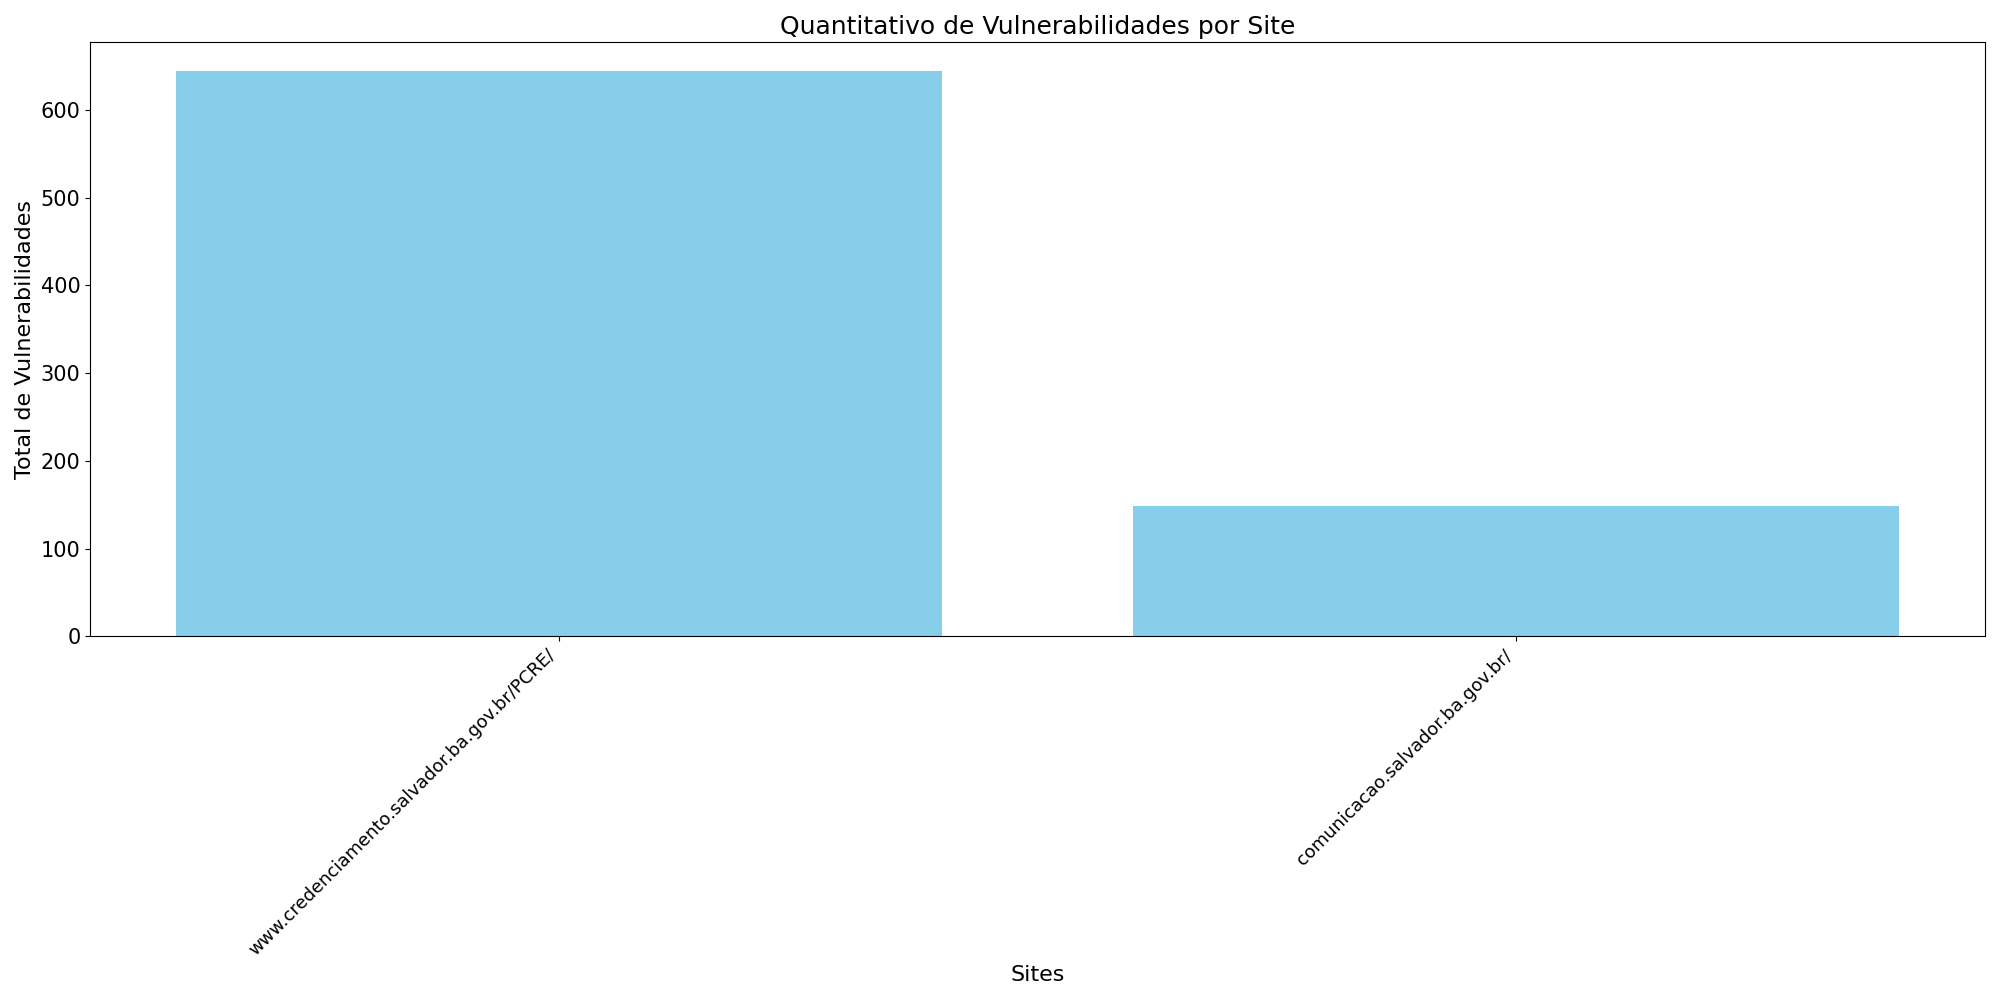
\includegraphics[width=1.0\textwidth]{assets/images-was/Vulnerabilidades_x_site.png}
    \caption{Total de vulnerabilidades por site}
\end{figure}
\FloatBarrier
As vulnerabilidades identificadas foram organizadas em seções e subseções, com o intuito de agrupá-las de acordo com sua afinidade e severidade. Cada seção aborda um conjunto específico de falhas de segurança, desde as relacionadas à configuração de segurança dos protocolos HTTP e TLS, até questões relacionadas à configuração inadequada do servidor e à exposição desnecessária de informações sensíveis. As subseções detalham vulnerabilidades em áreas como segurança de cookies e sessões, injeções de código, falhas de autenticação, entre outras. Essa estrutura facilita a análise, permitindo uma compreensão clara dos riscos e das recomendações de mitigação associadas a cada tipo de vulnerabilidade identificada.

%-------------- INÍCIO DA CATEGORIA Vulnerabilidades Relacionadas a Configurações de Segurança HTTP E TLS --------------
%-------------- INÍCIO DA CATEGORIA Vulnerabilidades Relacionadas a Configurações de Segurança HTTP E TLS --------------
\subsection{Vulnerabilidades Relacionadas a Configurações de Segurança HTTP E TLS}
Esta categoria aborda as vulnerabilidades associadas à configuração inadequada ou ausente de medidas de segurança no protocolo HTTP e na implementação de TLS, cruciais para a proteção da comunicação entre o cliente e o servidor.

%-------------- INÍCIO DA SUBCATEGORIA Informações de Cabeçalho --------------
\subsubsection{Informações de Cabeçalho}
Descrição não disponível.

\begin{enumerate}
%-------------- INÍCIO DA VULNERABILIDADE HTTP Header Information Disclosure --------------
\item \textbf{\texttt{HTTP Header Information Disclosure}}

                        \begin{figure}[h!]
                        \centering
                        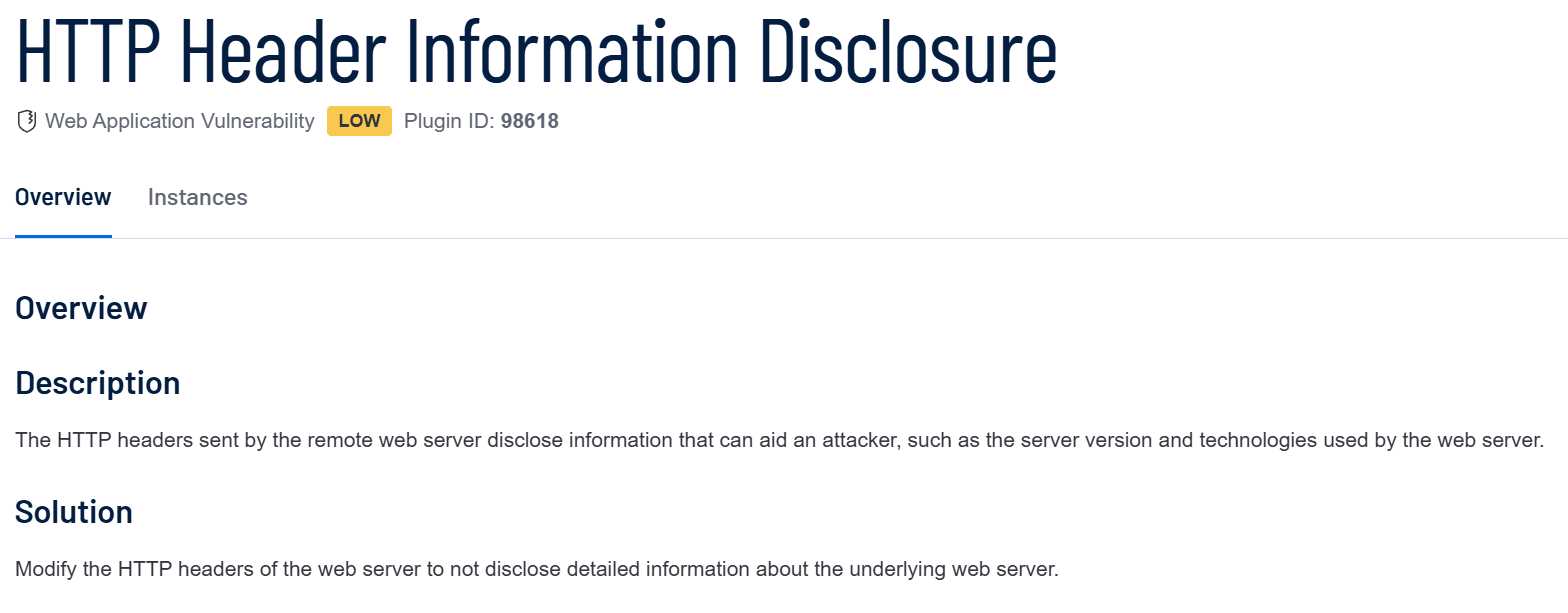
\includegraphics[width=0.8\textwidth]{assets/images-was/Vulnerabilidades Relacionadas a Configurações de Segurança HTTP E TLS/HTTP_header_Information_disclosure.png}
                        \end{figure}
                        \FloatBarrier
                        \textbf{Descrição:} A vulnerabilidade de divulgação de informações em cabeçalhos HTTP ocorre quando o servidor web remoto envia cabeçalhos que revelam detalhes sensíveis, como a versão do servidor e as tecnologias utilizadas. Essas informações podem ser exploradas por um atacante para identificar potenciais pontos fracos ou vulnerabilidades específicas, facilitando a execução de ataques direcionados.

    É crucial que as organizações implementem práticas de segurança, como a minimização das informações expostas nos cabeçalhos HTTP, para reduzir o risco de exploração. A configuração adequada do servidor pode mitigar a divulgação desnecessária de dados que possam ser utilizados para comprometer a segurança da aplicação.

\textbf{Solução:} Para mitigar essa vulnerabilidade, recomendamos a modificação dos cabeçalhos HTTP do servidor web para não divulgar informações detalhadas sobre o servidor subjacente. A desativação ou modificação de cabeçalhos como Server, X-Powered-By, X-AspNet-Version e outros cabeçalhos que revelam a versão ou a tecnologia do servidor é essencial.

\textbf{Total de URIs Afetadas:} None

\textbf{URIs Afetadas:}
\begin{itemize}
    \item \url{https://comunicacao.salvador.ba.gov.br}
    \item \url{https://www.credenciamento.salvador.ba.gov.br}
\end{itemize}

%-------------- FIM DA VULNERABILIDADE HTTP Header Information Disclosure --------------
%-------------- INÍCIO DA VULNERABILIDADE Missing 'Cache-Control' Header --------------
\item \textbf{\texttt{Missing 'Cache-Control' Header}}

                        \begin{figure}[h!]
                        \centering
                        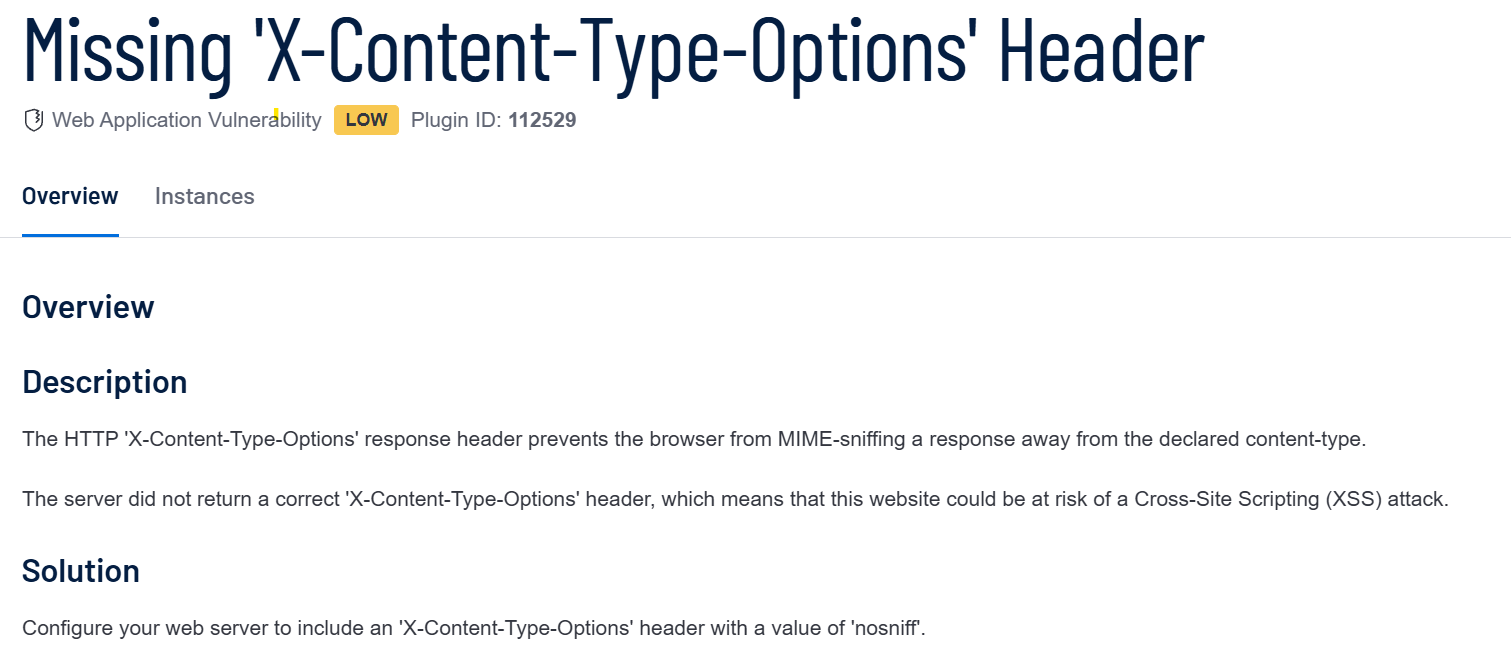
\includegraphics[width=0.8\textwidth]{assets/images-was/Vulnerabilidades Relacionadas a Configurações de Segurança HTTP E TLS/Missing 'X-Content-Type-Options' Header.png}
                        \end{figure}
                        \FloatBarrier
                        \textbf{Descrição:} A vulnerabilidade relacionada à ausência do cabeçalho X-Frame-Options ocorre quando o servidor web não envia o cabeçalho HTTP que define se a página pode ou não ser exibida em um frame ou iframe. Isso pode tornar o site vulnerável a ataques de clickjacking, onde um atacante manipula a interface do usuário para enganá-lo a clicar em algo diferente do que ele percebia, visando revelar informações confidenciais ou tomar controle do computador do usuário.

    A ausência do cabeçalho X-Frame-Options significa que o site pode ser incorporado em frames de outros sites, expondo os usuários a riscos de clickjacking. A implementação deste cabeçalho é uma medida importante para proteger os usuários contra esse tipo de ataque.

\textbf{Solução:} Para mitigar essa vulnerabilidade, recomenda-se configurar o servidor web para incluir o cabeçalho X-Frame-Options em todas as respostas HTTP. Isso pode ser feito configurando o servidor para permitir ou bloquear a exibição da página em frames, sendo recomendado o valor DENY ou SAMEORIGIN para evitar que o conteúdo seja incorporado em sites de terceiros.

\textbf{Total de URIs Afetadas:} None

\textbf{URIs Afetadas:}
\begin{itemize}
    \item \url{https://comunicacao.salvador.ba.gov.br}
    \item \url{https://www.credenciamento.salvador.ba.gov.br}
\end{itemize}

%-------------- FIM DA VULNERABILIDADE Missing 'Cache-Control' Header --------------
%-------------- INÍCIO DA VULNERABILIDADE Missing 'Content-Type' Header --------------
\item \textbf{\texttt{Missing 'Content-Type' Header}}

                        \begin{figure}[h!]
                        \centering
                        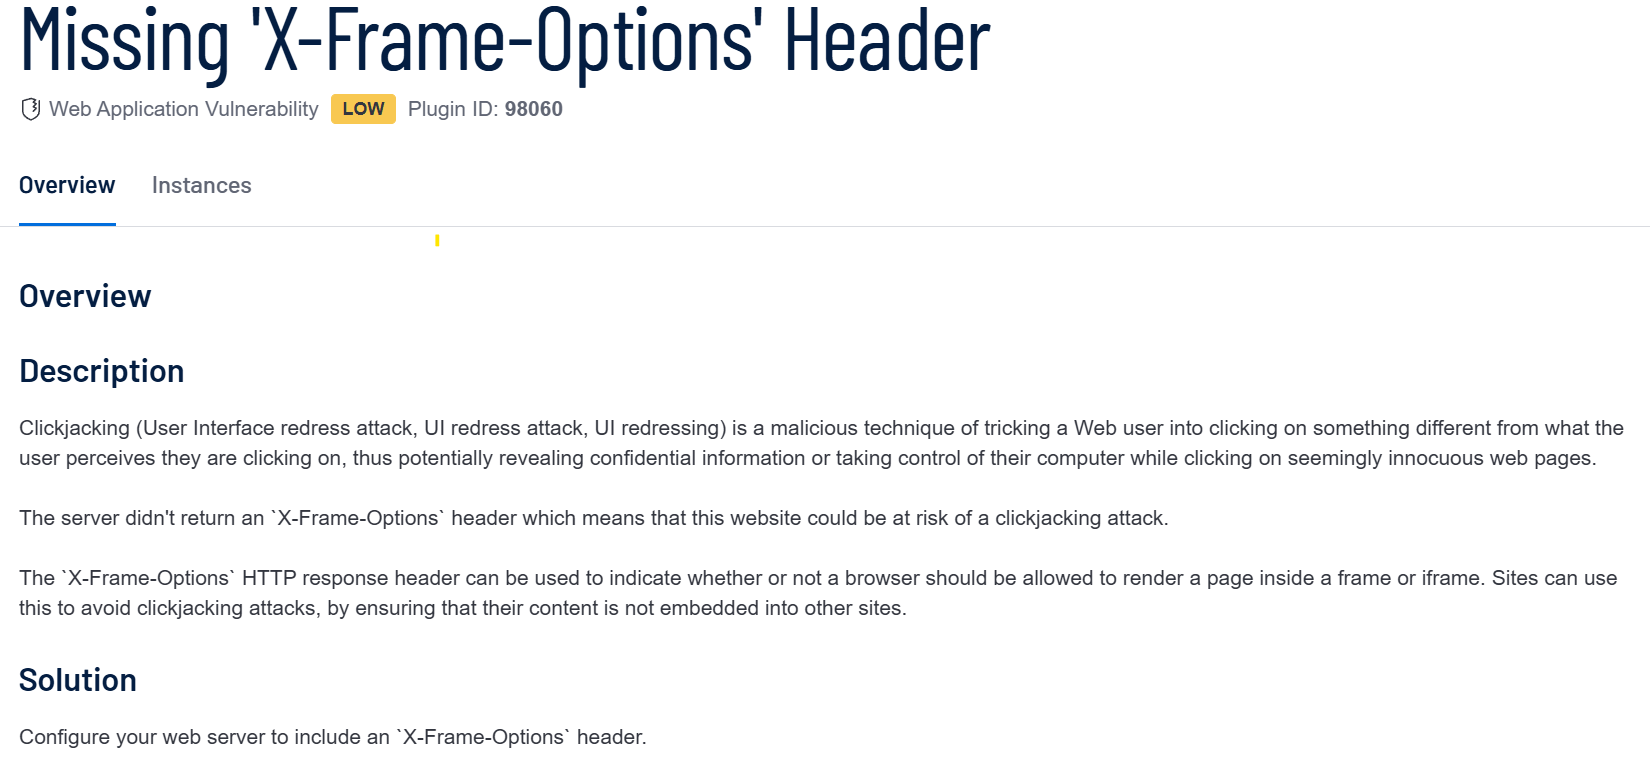
\includegraphics[width=0.8\textwidth]{assets/images-was/Vulnerabilidades Relacionadas a Configurações de Segurança HTTP E TLS/Missing 'X-Frame-Options' Header.png}
                        \end{figure}
                        \FloatBarrier
                        \textbf{Descrição:} A vulnerabilidade de ausência do cabeçalho X-Frame-Options ocorre quando o servidor web não retorna esse cabeçalho nas respostas HTTP. O cabeçalho X-Frame-Options é crucial para proteger os usuários contra ataques de clickjacking, um tipo de ataque onde o atacante engana o usuário a clicar em um elemento diferente do que ele percebe, frequentemente resultando na execução de ações não intencionais, como a revelação de informações confidenciais ou o controle do computador do usuário.

    Sem a presença do cabeçalho X-Frame-Options, o conteúdo do site pode ser carregado em um frame ou iframe de outro site, o que facilita a exploração dessa vulnerabilidade. Isso ocorre porque um atacante pode embutir o site vulnerável em um iframe disfarçado, enganando o usuário a clicar em botões ou links que, na realidade, estão direcionados para outra ação maliciosa.

\textbf{Solução:} Para mitigar esse risco, recomenda-se configurar o servidor web para incluir o cabeçalho X-Frame-Options nas respostas HTTP. Esse cabeçalho pode ser configurado para bloquear a exibição da página em frames de outros sites, utilizando o valor DENY (proibindo completamente) ou SAMEORIGIN (permitindo apenas a exibição no mesmo domínio). Essa simples configuração ajuda a evitar que o conteúdo do site seja incorporado em páginas de terceiros, protegendo os usuários contra ataques de clickjacking.

\textbf{Total de URIs Afetadas:} None

\textbf{URIs Afetadas:}
\begin{itemize}
    \item \url{https://www.credenciamento.salvador.ba.gov.br}
\end{itemize}

%-------------- FIM DA VULNERABILIDADE Missing 'Content-Type' Header --------------
%-------------- INÍCIO DA VULNERABILIDADE Missing 'X-Content-Type-Options' Header --------------
\item \textbf{\texttt{Missing 'X-Content-Type-Options' Header}}

                        \begin{figure}[h!]
                        \centering
                        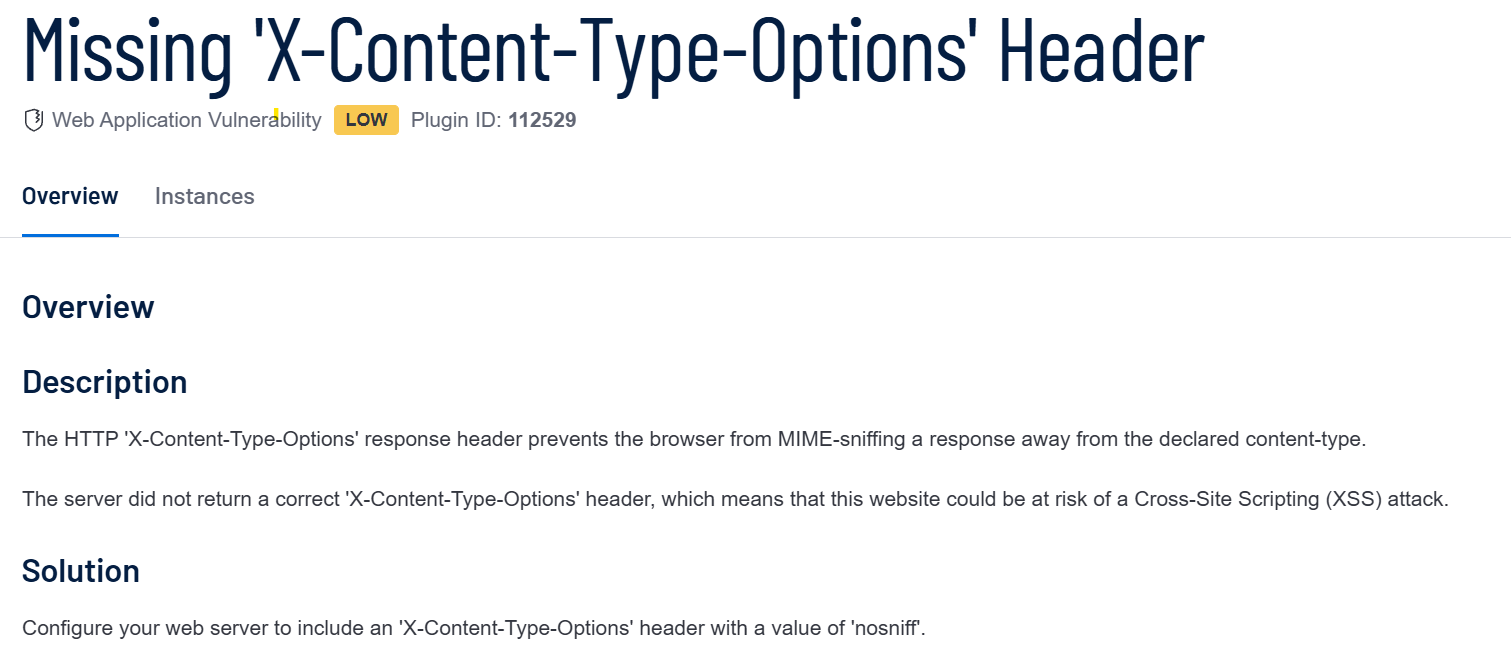
\includegraphics[width=0.8\textwidth]{assets/images-was/Vulnerabilidades Relacionadas a Configurações de Segurança HTTP E TLS/Missing 'X-Content-Type-Options' Header.png}
                        \end{figure}
                        \FloatBarrier
                        \textbf{Descrição:} A vulnerabilidade relacionada à ausência do cabeçalho X-Frame-Options ocorre quando o servidor web não envia o cabeçalho HTTP que define se a página pode ou não ser exibida em um frame ou iframe. Isso pode tornar o site vulnerável a ataques de clickjacking, onde um atacante manipula a interface do usuário para enganá-lo a clicar em algo diferente do que ele percebia, visando revelar informações confidenciais ou tomar controle do computador do usuário. A ausência do cabeçalho X-Frame-Options significa que o site pode ser incorporado em frames de outros sites, expondo os usuários a riscos de clickjacking. A implementação deste cabeçalho é uma medida importante para proteger os usuários contra esse tipo de ataque.

\textbf{Solução:} Para mitigar essa vulnerabilidade, recomenda-se configurar o servidor web para incluir o cabeçalho X-Frame-Options em todas as respostas HTTP. Isso pode ser feito configurando o servidor para permitir ou bloquear a exibição da página em frames, sendo recomendado o valor DENY ou SAMEORIGIN para evitar que o conteúdo seja incorporado em sites de terceiros.

\textbf{Total de URIs Afetadas:} None

\textbf{URIs Afetadas:}
\begin{itemize}
    \item \url{https://www.credenciamento.salvador.ba.gov.br}
\end{itemize}

%-------------- FIM DA VULNERABILIDADE Missing 'X-Content-Type-Options' Header --------------
%-------------- INÍCIO DA VULNERABILIDADE Missing 'X-Frame-Options' Header --------------
\item \textbf{\texttt{Missing 'X-Frame-Options' Header}}

                        \begin{figure}[h!]
                        \centering
                        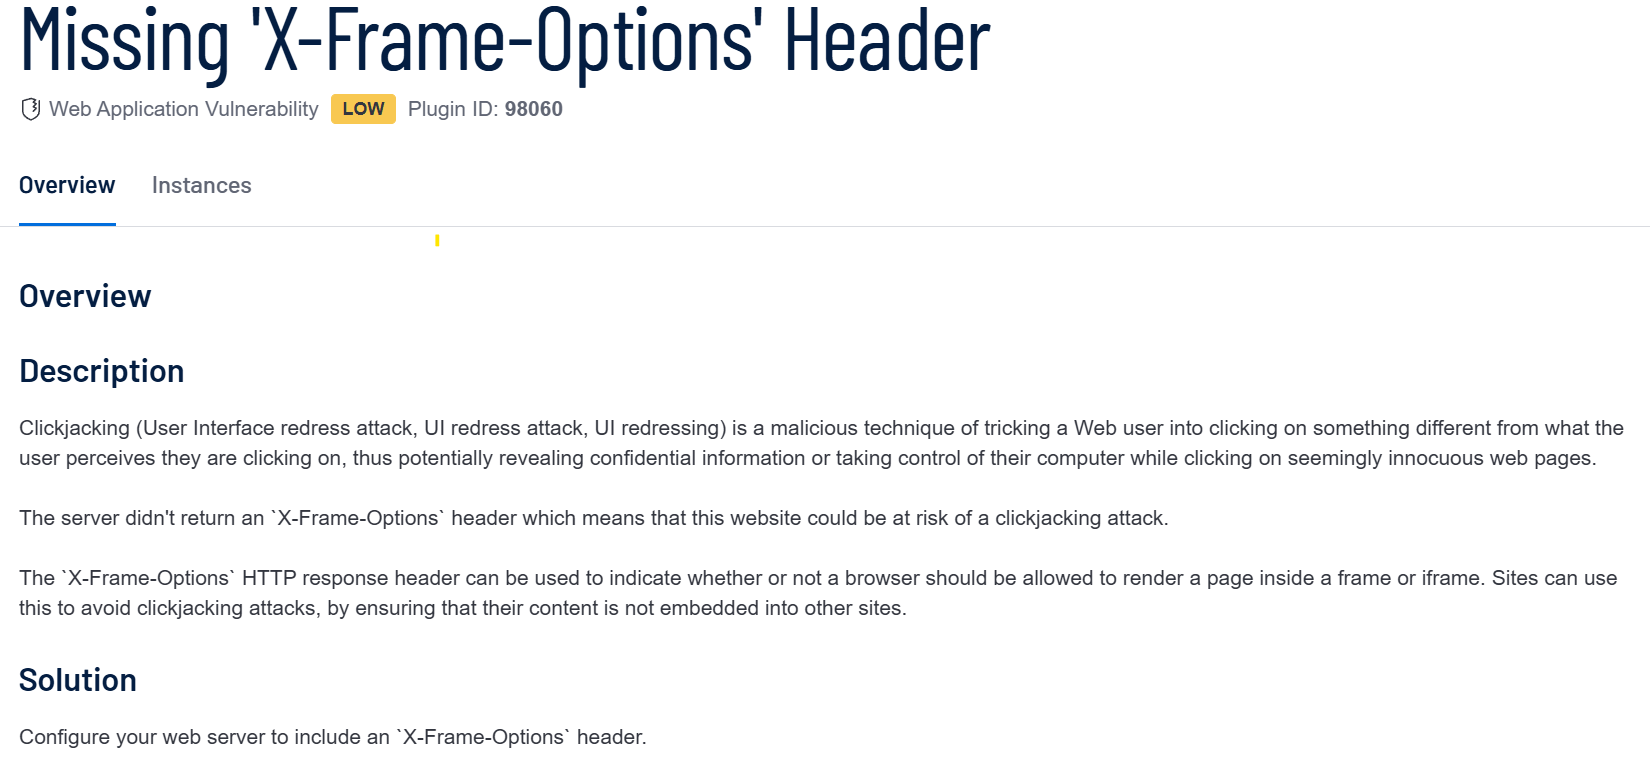
\includegraphics[width=0.8\textwidth]{assets/images-was/Vulnerabilidades Relacionadas a Configurações de Segurança HTTP E TLS/Missing 'X-Frame-Options' Header.png}
                        \end{figure}
                        \FloatBarrier
                        \textbf{Descrição:} A vulnerabilidade de ausência do cabeçalho X-Frame-Options ocorre quando o servidor web não retorna esse cabeçalho nas respostas HTTP. O cabeçalho X-Frame-Options é crucial para proteger os usuários contra ataques de clickjacking, um tipo de ataque onde o atacante engana o usuário a clicar em um elemento diferente do que ele percebe, frequentemente resultando na execução de ações não intencionais, como a revelação de informações confidenciais ou o controle do computador do usuário.

Sem a presença do cabeçalho X-Frame-Options, o conteúdo do site pode ser carregado em um frame ou iframe de outro site, o que facilita a exploração dessa vulnerabilidade. Isso ocorre porque um atacante pode embutir o site vulnerável em um iframe disfarçado, enganando o usuário a clicar em botões ou links que, na realidade, estão direcionados para outra ação maliciosa.

\textbf{Solução:} Para mitigar esse risco, recomenda-se configurar o servidor web para incluir o cabeçalho X-Frame-Options nas respostas HTTP. Esse cabeçalho pode ser configurado para bloquear a exibição da página em frames de outros sites, utilizando o valor DENY (proibindo completamente) ou SAMEORIGIN (permitindo apenas a exibição no mesmo domínio). Essa simples configuração ajuda a evitar que o conteúdo do site seja incorporado em páginas de terceiros, protegendo os usuários contra ataques de clickjacking.

\textbf{Total de URIs Afetadas:} None

\textbf{URIs Afetadas:}
\begin{itemize}
    \item \url{https://comunicacao.salvador.ba.gov.br}
\end{itemize}

%-------------- FIM DA VULNERABILIDADE Missing 'X-Frame-Options' Header --------------
%-------------- INÍCIO DA VULNERABILIDADE Missing Content Security Policy --------------
\item \textbf{\texttt{Missing Content Security Policy}}

                        \begin{figure}[h!]
                        \centering
                        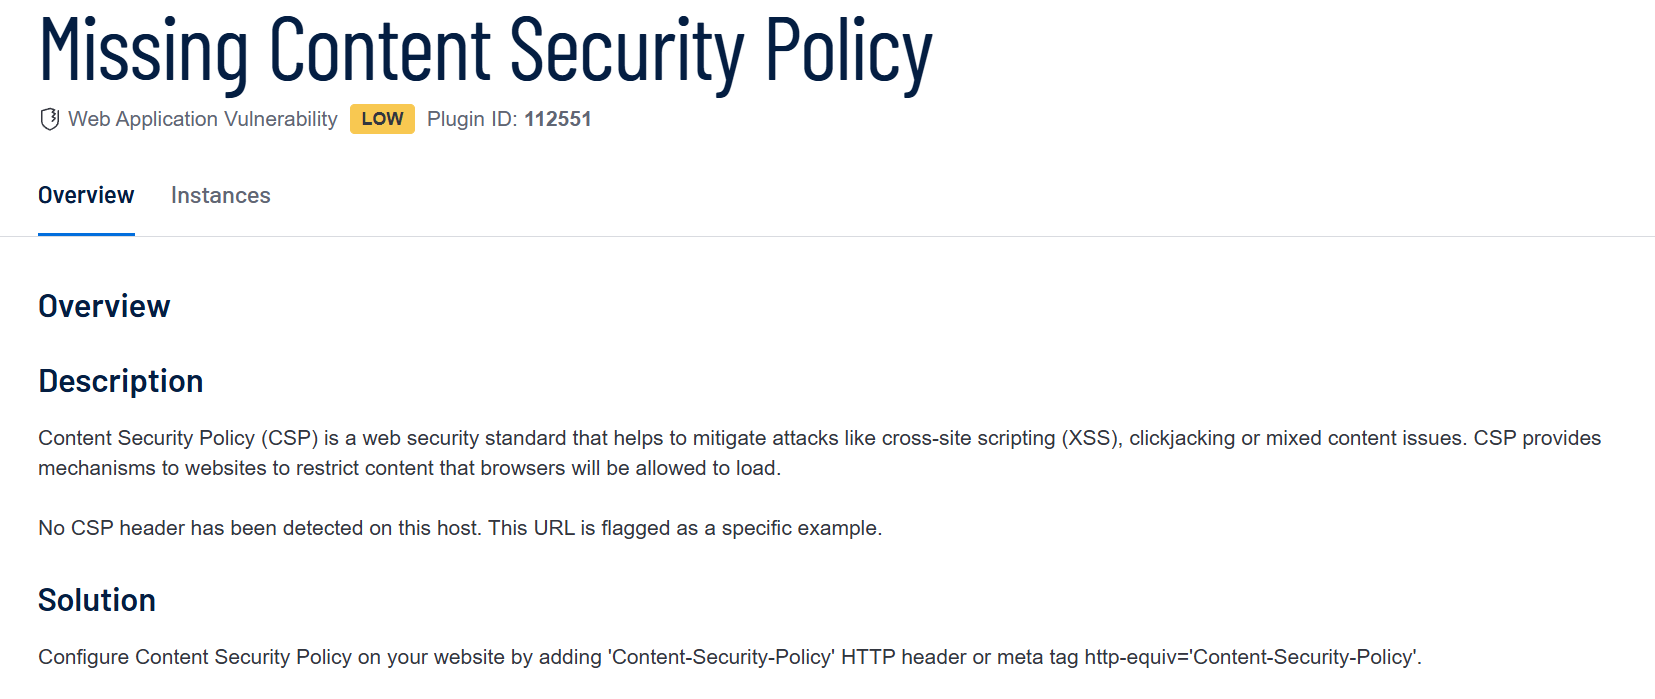
\includegraphics[width=0.8\textwidth]{assets/images-was/Vulnerabilidades Relacionadas a Configurações de Segurança HTTP E TLS/Missing Content Security Policy.png}
                        \end{figure}
                        \FloatBarrier
                        \textbf{Descrição:} A Política de Segurança de Conteúdo (CSP) é um padrão de segurança da web que ajuda a mitigar ataques como Cross-Site Scripting (XSS), clickjacking ou problemas de conteúdo misto. O CSP fornece mecanismos para que os sites restrinjam o conteúdo que os navegadores podem carregar.
 Nenhum cabeçalho CSP foi detectado neste host. Esta URL é sinalizada como um exemplo específico.

\textbf{Solução:} Configure a Política de Segurança de Conteúdo no seu site, adicionando o cabeçalho HTTP 'Content-Security-Policy' ou a tag meta http-equiv='Content-Security-Policy'.

\textbf{Total de URIs Afetadas:} None

\textbf{URIs Afetadas:}
\begin{itemize}
    \item \url{https://www.credenciamento.salvador.ba.gov.br}
\end{itemize}

%-------------- FIM DA VULNERABILIDADE Missing Content Security Policy --------------
%-------------- INÍCIO DA VULNERABILIDADE Missing HTTP Strict Transport Security Policy --------------
\item \textbf{\texttt{Missing HTTP Strict Transport Security Policy}}

                        \begin{figure}[h!]
                        \centering
                        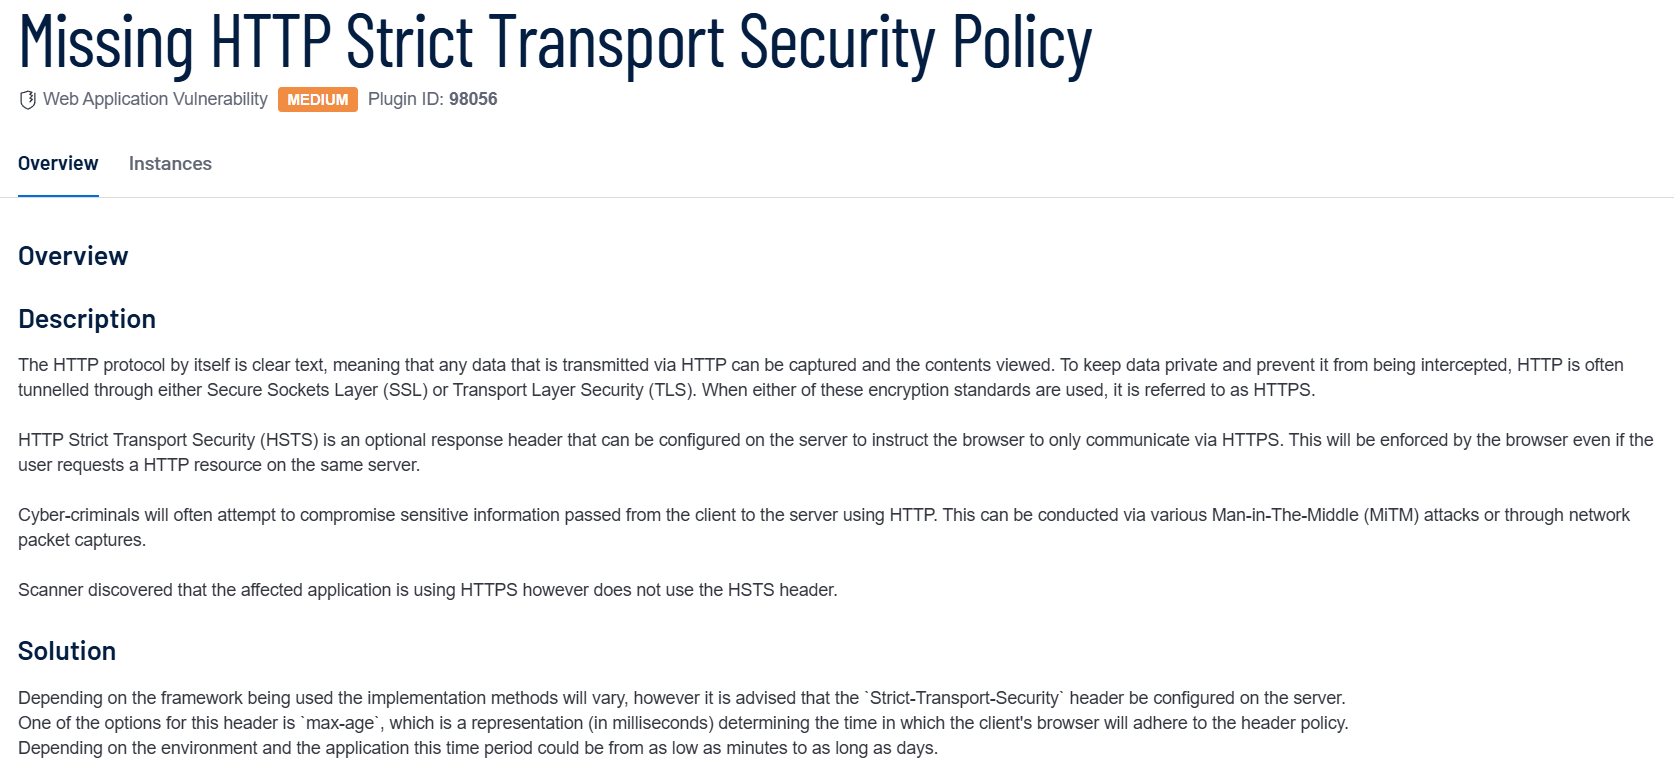
\includegraphics[width=0.8\textwidth]{assets/images-was/Vulnerabilidades Relacionadas a Configurações de Segurança HTTP E TLS/Missing HTTP Strict Transport Security Policy.png}
                        \end{figure}
                        \FloatBarrier
                        \textbf{Descrição:} O protocolo HTTP transmite dados em texto claro, o que significa que qualquer dado enviado via HTTP pode ser interceptado e visualizado. Para proteger a privacidade e evitar a interceptação de dados, o HTTP é frequentemente encapsulado através dos padrões de criptografia Secure Sockets Layer (SSL) ou Transport Layer Security (TLS), resultando no uso de HTTPS.

O HTTP Strict Transport Security (HSTS) é um cabeçalho de resposta opcional que pode ser configurado no servidor para instruir o navegador a se comunicar exclusivamente via HTTPS. Essa política será forçada pelo navegador, mesmo que o usuário tente acessar um recurso HTTP na mesma origem. O HSTS ajuda a proteger contra ataques de downgrade, em que um atacante pode tentar forçar uma conexão insegura em vez de usar a versão segura HTTPS.

Criminosos cibernéticos costumam tentar comprometer informações sensíveis transmitidas entre o cliente e o servidor via HTTP, utilizando técnicas como ataques Man-in-The-Middle (MiTM) ou capturas de pacotes de rede. Embora a aplicação afetada utilize HTTPS, ela não está utilizando o cabeçalho HSTS, o que a deixa vulnerável a esse tipo de ataque.

\textbf{Solução:} Para mitigar esse risco, é altamente recomendado configurar o cabeçalho Strict-Transport-Security no servidor. Esse cabeçalho instrui os navegadores a forçar o uso do HTTPS e a garantir que, mesmo que o usuário tente acessar uma versão HTTP de um recurso, a comunicação será automaticamente redirecionada para HTTPS. Uma das opções para configurar o cabeçalho é o parâmetro max-age, que define o tempo (em segundos) pelo qual o navegador deve seguir a política de HSTS. O período pode variar conforme o ambiente e os requisitos da aplicação, podendo ser de alguns minutos até vários dias.

\textbf{Total de URIs Afetadas:} None

\textbf{URIs Afetadas:}
\begin{itemize}
    \item \url{https://www.credenciamento.salvador.ba.gov.br}
\end{itemize}

%-------------- FIM DA VULNERABILIDADE Missing HTTP Strict Transport Security Policy --------------
%-------------- INÍCIO DA VULNERABILIDADE Mixed Resource Detection --------------
\item \textbf{\texttt{Mixed Resource Detection}}

                        \begin{figure}[h!]
                        \centering
                        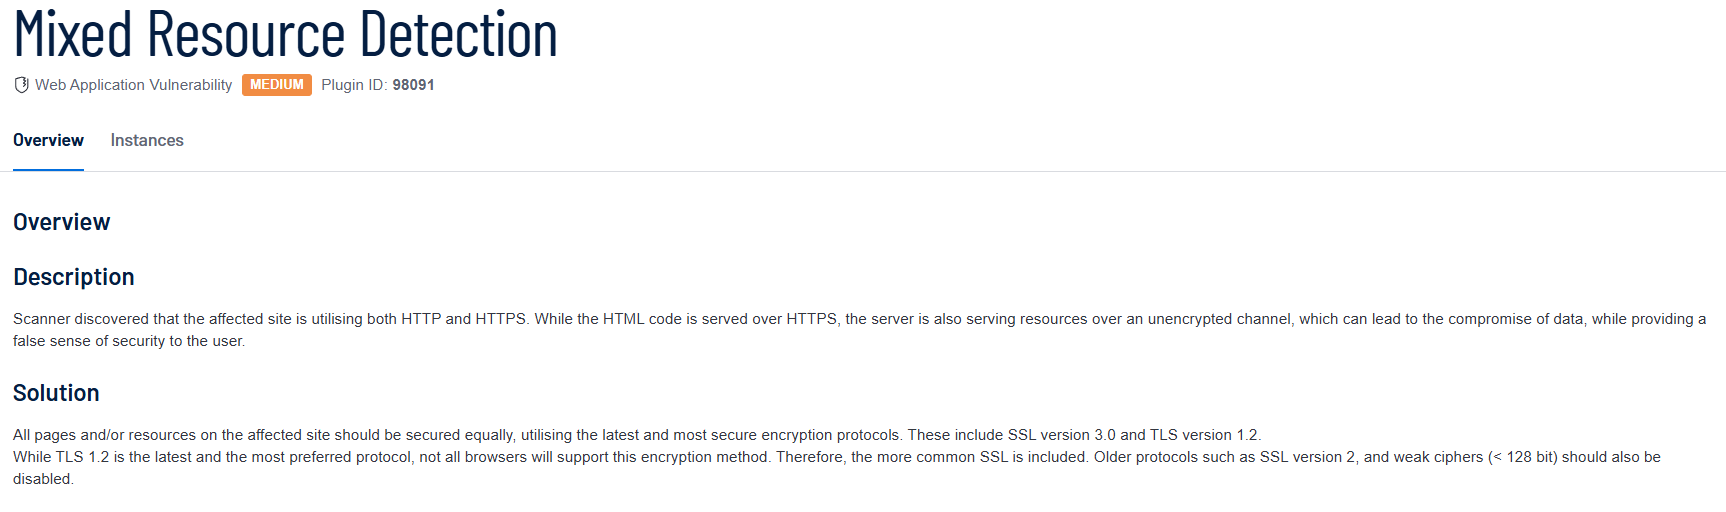
\includegraphics[width=0.8\textwidth]{assets/images-was/Vulnerabilidades Relacionadas a Configurações de Segurança HTTP E TLS/Mixed Resource Detection}
                        \end{figure}
                        \FloatBarrier
                        \textbf{Descrição:} O scanner descobriu que o site afetado está utilizando tanto HTTP quanto HTTPS. Embora o código HTML seja servido via HTTPS, o servidor também está fornecendo recursos por um canal não criptografado, o que pode comprometer os dados, ao mesmo tempo que oferece uma falsa sensação de segurança ao usuário.


\textbf{Solução:} Todas as páginas e/ou recursos no site afetado devem ser igualmente protegidos, utilizando os protocolos de criptografia mais seguros e recentes, como TLS 1.2 e TLS 1.3.

\textbf{Total de URIs Afetadas:} None

\textbf{URIs Afetadas:}
\begin{itemize}
    \item \url{https://www.credenciamento.salvador.ba.gov.br}
\end{itemize}

%-------------- FIM DA VULNERABILIDADE Mixed Resource Detection --------------
%-------------- INÍCIO DA VULNERABILIDADE Permissive Content Security Policy Detected --------------
\item \textbf{\texttt{Permissive Content Security Policy Detected}}

                        \begin{figure}[h!]
                        \centering
                        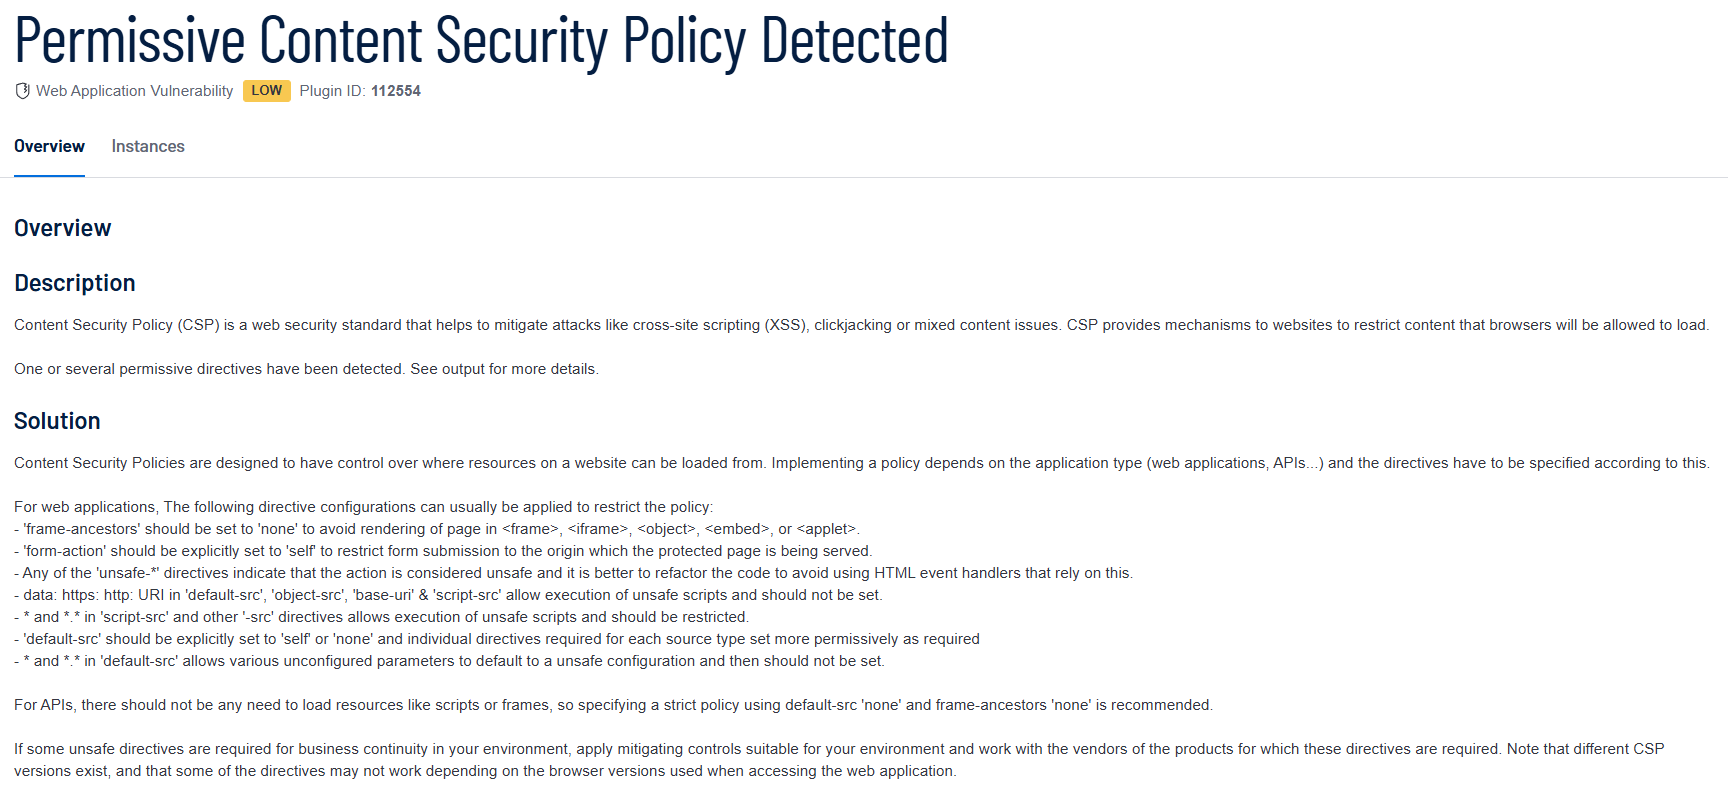
\includegraphics[width=0.8\textwidth]{assets/images-was/Outras Vulnerabilidades Críticas e Explorações/Desafios de Configuração de Segurança/Permissive Content Security Policy Detected.png}
                        \end{figure}
                        \FloatBarrier
                        \textbf{Descrição:} A Política de Segurança de Conteúdo (CSP) é um padrão de segurança da web que ajuda a mitigar ataques como Cross-Site Scripting (XSS), clickjacking ou problemas de conteúdo misto. O CSP permite que os sites controlem quais recursos os navegadores podem carregar, restringindo o conteúdo carregado e aumentando a proteção contra ataques.

No entanto, uma política de CSP excessivamente permissiva pode permitir que conteúdos não seguros sejam carregados, o que enfraquece a eficácia da política. O scanner identificou uma ou mais diretivas permissivas na política de CSP do site, o que pode expor o site a ataques como injeção de scripts maliciosos (XSS), carregamento de conteúdo inseguro ou execução de código não autorizado.

As diretivas permissivas podem incluir, por exemplo, o uso de * ou *.* nas diretrizes de fontes (como script-src ou default-src), o que permite a execução de scripts ou o carregamento de recursos de origens não confiáveis. Isso pode comprometer a segurança da aplicação ao permitir a execução de código arbitrário proveniente de fontes não autorizadas.

\textbf{Solução:} Para corrigir essa vulnerabilidade, recomenda-se restringir a política de CSP e aplicar as diretivas de forma mais rígida. A seguir, estão algumas diretrizes gerais que podem ser implementadas:

- Defina frame-ancestors como none para evitar que a página seja renderizada dentro de <frame>, <iframe>, <object>, <embed> ou <applet>.
- Configure form-action explicitamente como self para restringir o envio de formulários apenas à origem do site.
- Evite o uso das diretivas unsafe-*, pois indicam ações inseguras. Refatore o código para não depender de manipuladores de eventos HTML que utilizem essas diretivas.
- Evite o uso de data:, https: ou http: nas diretivas default-src, object-src, base-uri e script-src, pois essas configurações permitem a execução de scripts não seguros.
- Não utilize * ou *.* em diretivas como script-src e outras diretrizes -src, pois isso permite a execução de scripts não seguros de origens não especificadas.
- Defina default-src explicitamente como self ou none, e defina as diretivas individuais de forma mais permissiva apenas quando necessário.
- Para APIs, deve-se evitar carregar recursos como scripts ou frames. Use uma política rígida com default-src 'none' e frame-ancestors 'none'.

Se for necessário usar algumas diretivas inseguras para a continuidade dos negócios, aplique controles mitigadores adequados ao seu ambiente e consulte os fornecedores dos produtos que exigem essas diretivas. Lembre-se de que existem versões diferentes do CSP e que algumas diretivas podem não ser suportadas em versões de navegador mais antigas.

\textbf{Total de URIs Afetadas:} None

\textbf{URIs Afetadas:}
\begin{itemize}
    \item \url{https://comunicacao.salvador.ba.gov.br}
\end{itemize}

%-------------- FIM DA VULNERABILIDADE Permissive Content Security Policy Detected --------------
%-------------- INÍCIO DA VULNERABILIDADE Permissive HTTP Strict Transport Security Policy Detected --------------
\item \textbf{\texttt{Permissive HTTP Strict Transport Security Policy Detected}}

                        \begin{figure}[h!]
                        \centering
                        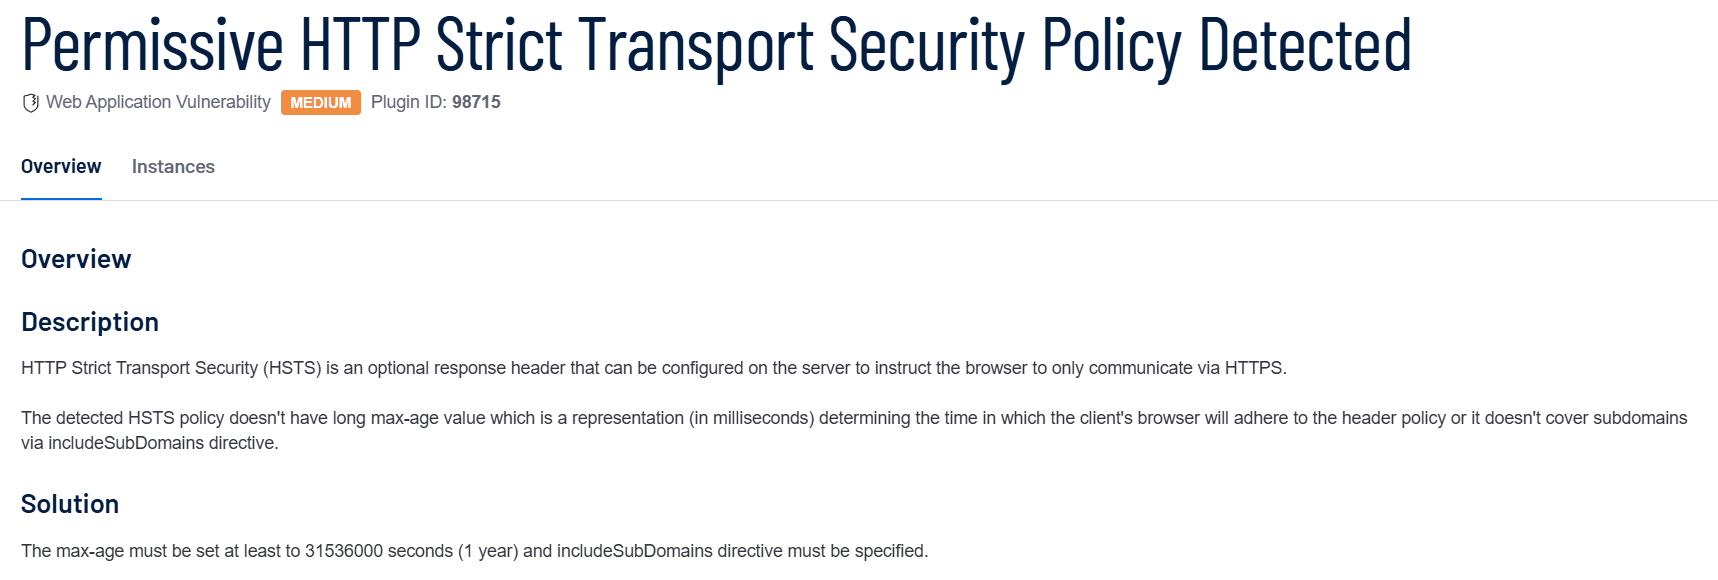
\includegraphics[width=0.8\textwidth]{assets/images-was/Vulnerabilidades Relacionadas a Configurações de Segurança HTTP E TLS/Permissive HTTP Strict Transport Security Policy Detected.png}
                        \end{figure}
                        \FloatBarrier
                        \textbf{Descrição:} O HTTP Strict Transport Security (HSTS) é um cabeçalho de resposta opcional que pode ser configurado no servidor para instruir o navegador a se comunicar exclusivamente via HTTPS. Ao ser configurado corretamente, o HSTS ajuda a proteger os usuários contra ataques de downgrade e interceptação de dados. No entanto, foi detectado que a política HSTS configurada para o servidor não possui um valor suficientemente longo para o parâmetro max-age ou não cobre subdomínios por meio da diretiva includeSubDomains.

\textbf{Solução:} Para melhorar a segurança e evitar que a política HSTS seja permissiva demais, é recomendado ajustar o parâmetro max-age para um valor de, pelo menos, 31536000 segundos (1 ano). Além disso, a diretiva includeSubDomains deve ser especificada para garantir que todos os subdomínios sejam protegidos pela mesma política HSTS.

\textbf{Total de URIs Afetadas:} None

\textbf{URIs Afetadas:}
\begin{itemize}
    \item \url{https://comunicacao.salvador.ba.gov.br}
\end{itemize}

%-------------- FIM DA VULNERABILIDADE Permissive HTTP Strict Transport Security Policy Detected --------------
\end{enumerate}
%-------------- FIM DA SUBCATEGORIA Informações de Cabeçalho --------------
%-------------- INÍCIO DA SUBCATEGORIA Protocolos e Cifragem --------------
\subsubsection{Protocolos e Cifragem}
Descrição não disponível.

\begin{enumerate}
%-------------- INÍCIO DA VULNERABILIDADE SSL/TLS Forward Secrecy Cipher Suites Not Supported --------------
\item \textbf{\texttt{SSL/TLS Forward Secrecy Cipher Suites Not Supported}}

                        \begin{figure}[h!]
                        \centering
                        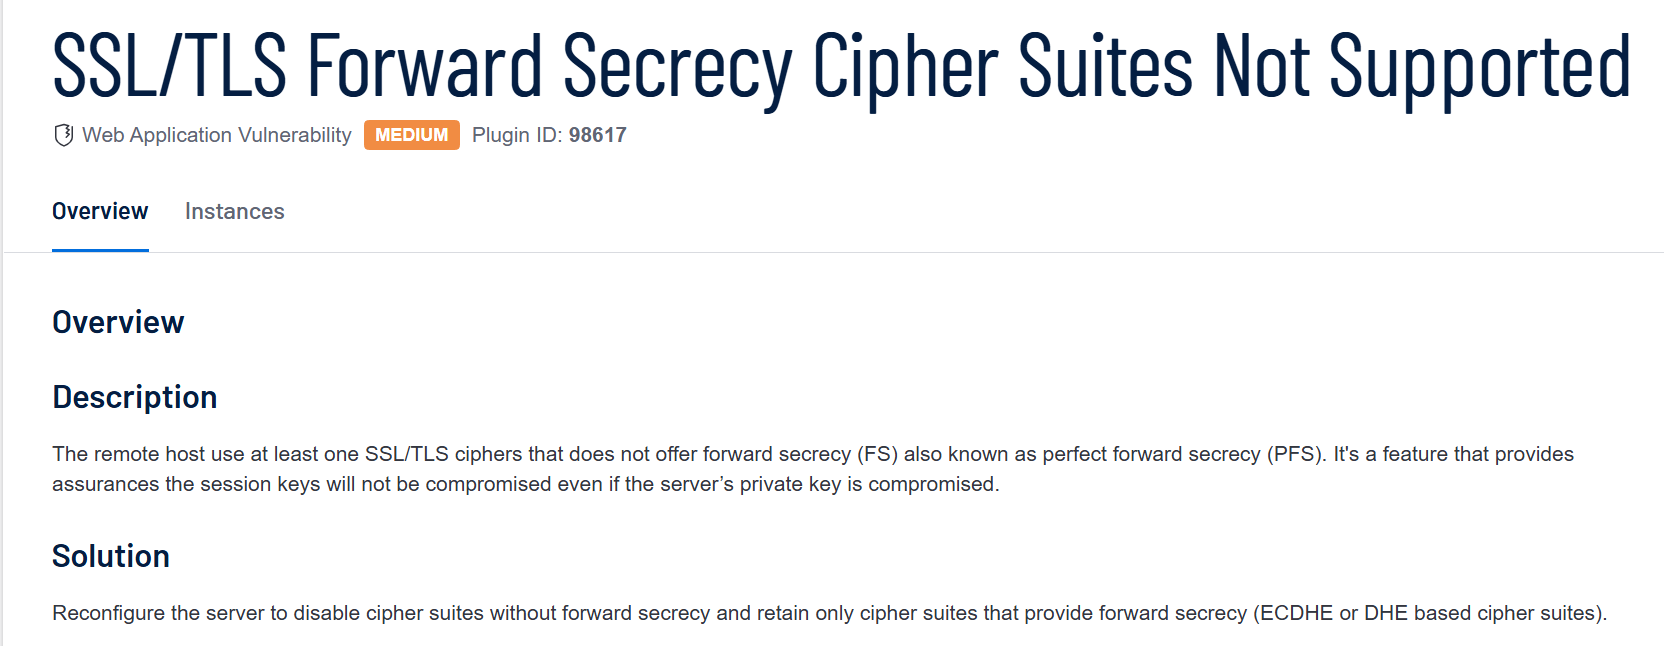
\includegraphics[width=0.8\textwidth]{assets/images-was/Protocolos e Cifragem/SSL-TLS Forward Secrecy Cipher Suites Not Supported}
                        \end{figure}
                        \FloatBarrier
                        \textbf{Descrição:} O host remoto utiliza pelo menos uma cifra SSL/TLS que não oferece segredo perfeito (FS), também conhecido como segredo perfeito de avanço (PFS). Essa é uma característica que garante que as chaves de sessão não serão comprometidas mesmo que a chave privada do servidor seja comprometida.


\textbf{Solução:} Reconfigure o servidor para desabilitar as cifras sem segredo perfeito e mantenha apenas as cifras que oferecem segredo perfeito (cifras baseadas em ECDHE ou DHE).

\textbf{Total de URIs Afetadas:} None

\textbf{URIs Afetadas:}
\begin{itemize}
    \item \url{https://comunicacao.salvador.ba.gov.br}
    \item \url{https://www.credenciamento.salvador.ba.gov.br}
\end{itemize}

%-------------- FIM DA VULNERABILIDADE SSL/TLS Forward Secrecy Cipher Suites Not Supported --------------
%-------------- INÍCIO DA VULNERABILIDADE SSL/TLS Weak Cipher Suites Supported --------------
\item \textbf{\texttt{SSL/TLS Weak Cipher Suites Supported}}

                        \begin{figure}[h!]
                        \centering
                        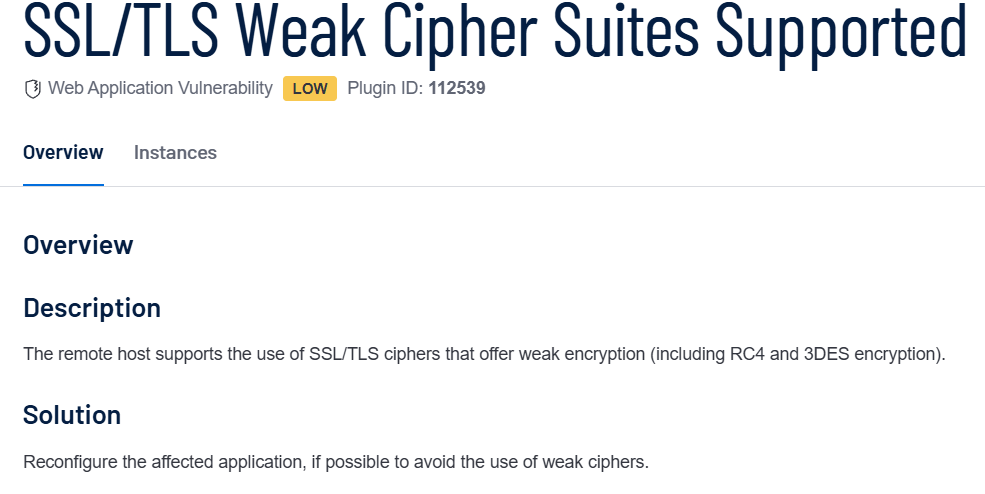
\includegraphics[width=0.8\textwidth]{assets/images-was/Protocolos e Cifragem/SSL-TLS Weak Cipher Suites Supported.png}
                        \end{figure}
                        \FloatBarrier
                        \textbf{Descrição:} O servidor remoto suporta o uso de conjuntos de cifras (cipher suites) de SSL/TLS que oferecem criptografia insegura, incluindo suites de exportação e cifras com menos de 128 bits. Esses conjuntos de cifras são considerados inseguros porque proporcionam um nível de proteção inadequado, tornando mais fácil para um atacante decifrar os dados transmitidos.

    Conjuntos de cifras com menos de 128 bits de força não oferecem uma barreira suficiente contra ataques de força bruta e outros métodos de comprometimento de dados. O suporte a essas cifras pode expor a comunicação a riscos significativos, incluindo a interceptação de dados sensíveis e a perda da integridade da transmissão.

\textbf{Solução:} Recomenda-se reconfigurar a aplicação ou servidor afetado para desabilitar o suporte a conjuntos de cifras fracas. As cifras mais seguras, como AES (Advanced Encryption Standard) em modos de operação modernos (por exemplo, GCM), devem ser priorizadas. Além disso, a configuração do servidor deve ser revisada para garantir o suporte a protocolos e algoritmos de criptografia que estejam de acordo com as melhores práticas de segurança, como TLS 1.2 ou TLS 1.3, que oferecem melhorias significativas em segurança e desempenho.

\textbf{Total de URIs Afetadas:} None

\textbf{URIs Afetadas:}
\begin{itemize}
    \item \url{https://comunicacao.salvador.ba.gov.br}
    \item \url{https://www.credenciamento.salvador.ba.gov.br}
\end{itemize}

%-------------- FIM DA VULNERABILIDADE SSL/TLS Weak Cipher Suites Supported --------------
\end{enumerate}
%-------------- FIM DA SUBCATEGORIA Protocolos e Cifragem --------------
%-------------- FIM DA CATEGORIA Vulnerabilidades Relacionadas a Configurações de Segurança HTTP E TLS --------------
%-------------- INÍCIO DA CATEGORIA Vulnerabilidades Relacionadas a Configurações e Exposição de Informações --------------
\subsection{Vulnerabilidades Relacionadas a Configurações e Exposição de Informações}
Esta categoria reúne vulnerabilidades associadas a configurações inadequadas do servidor e à exposição de informações sensíveis, que podem ser acessadas por atacantes devido à falta de medidas de segurança apropriadas.

%-------------- INÍCIO DA SUBCATEGORIA Exposição de Código e Recursos --------------
\subsubsection{Exposição de Código e Recursos}
Descrição não disponível.

\begin{enumerate}
%-------------- INÍCIO DA VULNERABILIDADE Source Code Passive Disclosure --------------
\item \textbf{\texttt{Source Code Passive Disclosure}}

                        \begin{figure}[h!]
                        \centering
                        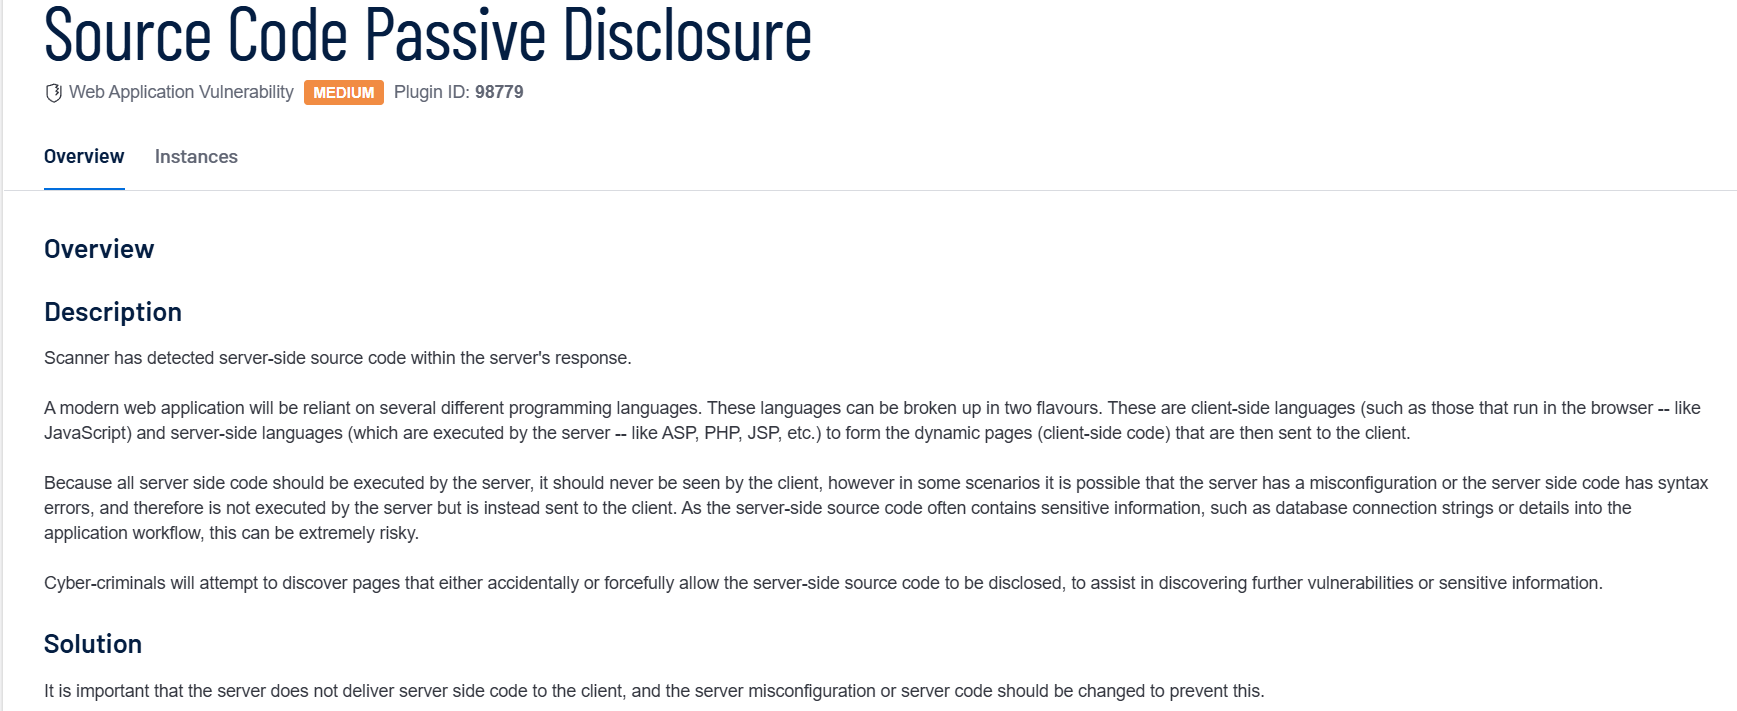
\includegraphics[width=0.8\textwidth]{assets/images-was/Vulnerabilidades Relacionadas a Configurações e Exposição de Informações/Exposição de Código e Recursos/Source Code Passive Disclosure.png}
                        \end{figure}
                        \FloatBarrier
                        \textbf{Descrição:} Foi detectada a divulgação passiva de código-fonte do lado do servidor na resposta do servidor. Aplicações web modernas utilizam diversas linguagens de programação que podem ser classificadas em duas categorias: linguagens do lado do cliente (executadas no navegador, como JavaScript) e linguagens do lado do servidor (executadas no servidor, como ASP, PHP, JSP, etc.), que formam as páginas dinâmicas enviadas ao cliente.

    Todo código do lado do servidor deve ser executado pelo servidor e nunca exposto ao cliente. No entanto, devido a configurações incorretas do servidor ou erros de sintaxe, pode ocorrer que o código do lado do servidor não seja executado e, em vez disso, seja enviado ao cliente. Como o código-fonte do lado do servidor frequentemente contém informações sensíveis, como strings de conexão de banco de dados ou detalhes sobre o fluxo de trabalho da aplicação, essa exposição representa um risco significativo.

    Criminosos cibernéticos podem tentar descobrir páginas que, acidentalmente ou propositalmente, permitem a divulgação do código-fonte do lado do servidor, a fim de identificar vulnerabilidades ou informações sensíveis.

\textbf{Solução:} É fundamental garantir que o servidor não entregue código do lado do servidor ao cliente. Para isso, deve-se corrigir a configuração incorreta do servidor ou ajustar o código do servidor para evitar essa exposição.

%---------------------------------------------------------------------------------
    \item

\textbf{Total de URIs Afetadas:} None

\textbf{URIs Afetadas:}
\begin{itemize}
    \item \url{https://comunicacao.salvador.ba.gov.br}
\end{itemize}

%-------------- FIM DA VULNERABILIDADE Source Code Passive Disclosure --------------
\end{enumerate}
%-------------- FIM DA SUBCATEGORIA Exposição de Código e Recursos --------------
%-------------- FIM DA CATEGORIA Vulnerabilidades Relacionadas a Configurações e Exposição de Informações --------------
%-------------- INÍCIO DA CATEGORIA Vulnerabilidades Relacionadas a Injeção de Código --------------
\subsection{Vulnerabilidades Relacionadas a Injeção de Código}
Esta categoria trata das vulnerabilidades de injeção de código, onde entradas de usuário não são devidamente validadas ou filtradas, permitindo a execução de código malicioso que pode comprometer a aplicação e os dados do usuário.

%-------------- INÍCIO DA SUBCATEGORIA Outras Injeções --------------
\subsubsection{Outras Injeções}
Descrição não disponível.

\begin{enumerate}
%-------------- INÍCIO DA VULNERABILIDADE HTML/CSS Injection --------------
\item \textbf{\texttt{HTML/CSS Injection}}

                        \begin{figure}[h!]
                        \centering
                        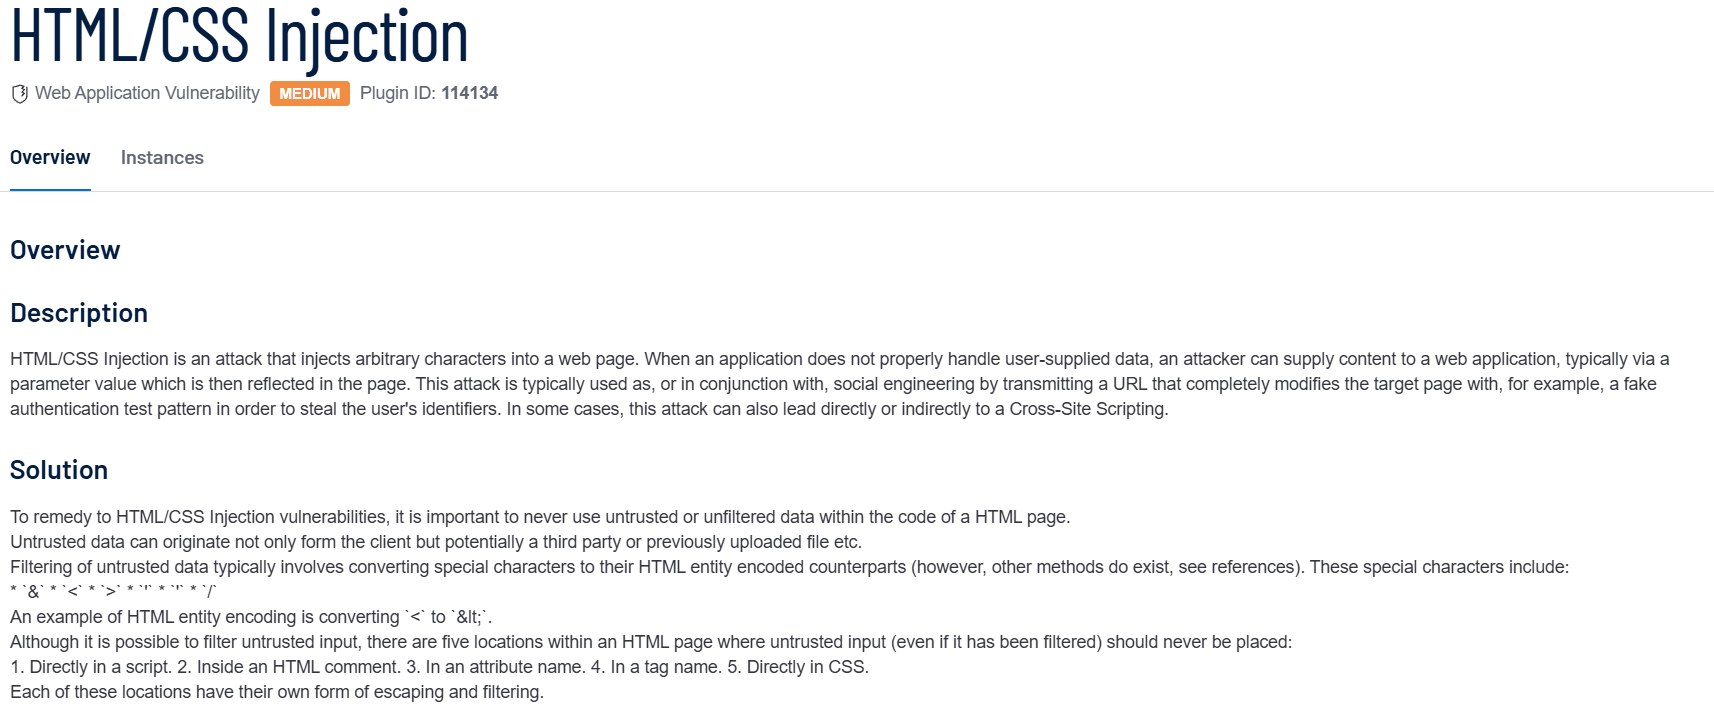
\includegraphics[width=0.8\textwidth]{assets/images-was/Vulnerabilidades Relacionadas a Injeção de Código/Outras Injeções/HTML-CSS Injection.png}
                        \end{figure}
                        \FloatBarrier
                        \textbf{Descrição:}  A injeção HTML/CSS é um ataque que injeta caracteres arbitrários em uma página web. Quando uma aplicação não lida corretamente com dados fornecidos pelo usuário, um atacante pode fornecer conteúdo a uma aplicação web, normalmente através de um valor de parâmetro que é refletido na página. Esse ataque é frequentemente usado como parte de engenharia social, transmitindo uma URL que modifica completamente a página alvo com, por exemplo, um padrão de teste de autenticação falso, para roubar os identificadores do usuário. Em alguns casos, esse ataque também pode levar, direta ou indiretamente, a um Cross-Site Scripting (XSS).


\textbf{Solução:} Para remediar as vulnerabilidades de injeção HTML/CSS, é importante nunca usar dados não confiáveis ou não filtrados dentro do código de uma página HTML.
Dados não confiáveis podem originar-se não apenas do cliente, mas também de terceiros ou de arquivos previamente carregados, entre outros.
A filtragem de dados não confiáveis normalmente envolve a conversão de caracteres especiais para suas versões codificadas em entidades HTML (no entanto, existem outros métodos, consulte as referências). Esses caracteres especiais incluem:
\begin{itemize}
    \item \texttt{\&}
    \item \texttt{<}
    \item \texttt{>}
    \item \texttt{\'}
    \item \texttt{\"}
    \item \texttt{/}
\end{itemize}
Um exemplo de codificação de entidades HTML é converter \texttt{<} para \texttt{\&lt;}.

Embora seja possível filtrar entradas não confiáveis, existem cinco locais dentro de uma página HTML onde a entrada não confiável (mesmo que filtrada) nunca deve ser colocada:
\begin{enumerate}
    \item Diretamente em um script.
    \item Dentro de um comentário HTML.
    \item Em um nome de atributo.
    \item Em um nome de tag.
    \item Diretamente em CSS.
\end{enumerate}
Cada um desses locais possui sua própria forma de escape e filtragem.

\textbf{Total de URIs Afetadas:} None

\textbf{URIs Afetadas:}
\begin{itemize}
    \item \url{https://comunicacao.salvador.ba.gov.br}
    \item \url{https://www.credenciamento.salvador.ba.gov.br}
\end{itemize}

%-------------- FIM DA VULNERABILIDADE HTML/CSS Injection --------------
\end{enumerate}
%-------------- FIM DA SUBCATEGORIA Outras Injeções --------------
%-------------- FIM DA CATEGORIA Vulnerabilidades Relacionadas a Injeção de Código --------------
%-------------- INÍCIO DA CATEGORIA Vulnerabilidades em Cookies e Segurança de Sessão --------------
\subsection{Vulnerabilidades em Cookies e Segurança de Sessão}
Esta categoria foca em vulnerabilidades relacionadas à segurança de cookies e sessões de usuário, essenciais para garantir que as informações de autenticação e sessão permaneçam protegidas contra roubo e ataques como fixação de sessão.

%-------------- INÍCIO DA SUBCATEGORIA Vulnerabilidades em Cookies e Segurança de Sessão --------------
\subsubsection{Vulnerabilidades em Cookies e Segurança de Sessão}
Descrição não disponível.

\begin{enumerate}
%-------------- INÍCIO DA VULNERABILIDADE Cookie Without HttpOnly Flag Detected --------------
\item \textbf{\texttt{Cookie Without HttpOnly Flag Detected}}

                        \begin{figure}[h!]
                        \centering
                        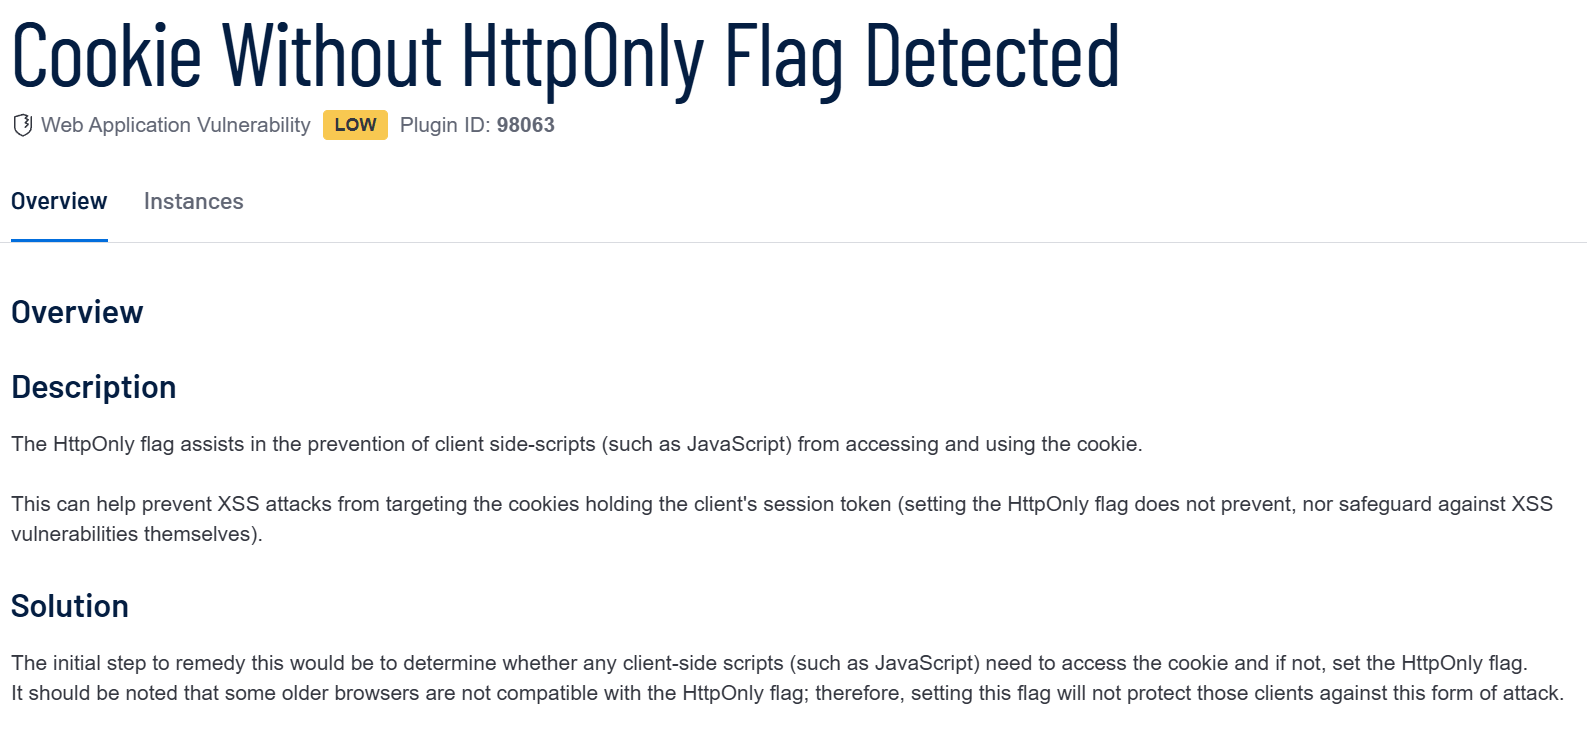
\includegraphics[width=0.8\textwidth]{assets/images-was/Vulnerabilidades em Cookies e Segurança de Sessão/Cookie Without HttpOnly Flag Detected.png}
                        \end{figure}
                        \FloatBarrier
                        \textbf{Descrição:} A flag \texttt{HttpOnly} ajuda a prevenir que scripts do lado do cliente (como o JavaScript) acessem e usem o cookie. Isso é particularmente importante para proteger os cookies que contêm tokens de sessão do cliente, já que impede que um script malicioso, como um que explora uma vulnerabilidade de Cross-Site Scripting (XSS), possa roubar esses dados sensíveis.

Vale destacar que configurar a flag \texttt{HttpOnly} não previne ou resolve vulnerabilidades XSS diretamente, mas limita o escopo de exploração ao impedir que os cookies sejam acessados por scripts do lado do cliente.

\textbf{Solução:} O primeiro passo para corrigir essa vulnerabilidade é determinar se algum script do lado do cliente (como o JavaScript) precisa acessar o cookie. Se o cookie não precisar ser acessado por scripts, a flag \texttt{HttpOnly} deve ser configurada. Essa configuração ajuda a proteger os dados do cookie contra tentativas de roubo por meio de ataques XSS.

É importante observar que navegadores mais antigos podem não ser compatíveis com a flag \texttt{HttpOnly}, o que significa que esses clientes ainda estarão suscetíveis a esse tipo de ataque, mesmo com a configuração da flag.

\textbf{Total de URIs Afetadas:} None

\textbf{URIs Afetadas:}
\begin{itemize}
    \item \url{https://comunicacao.salvador.ba.gov.br}
    \item \url{https://www.credenciamento.salvador.ba.gov.br}
\end{itemize}

%-------------- FIM DA VULNERABILIDADE Cookie Without HttpOnly Flag Detected --------------
%-------------- INÍCIO DA VULNERABILIDADE Cookie Without SameSite Flag Detected --------------
\item \textbf{\texttt{Cookie Without SameSite Flag Detected}}

                        \begin{figure}[h!]
                        \centering
                        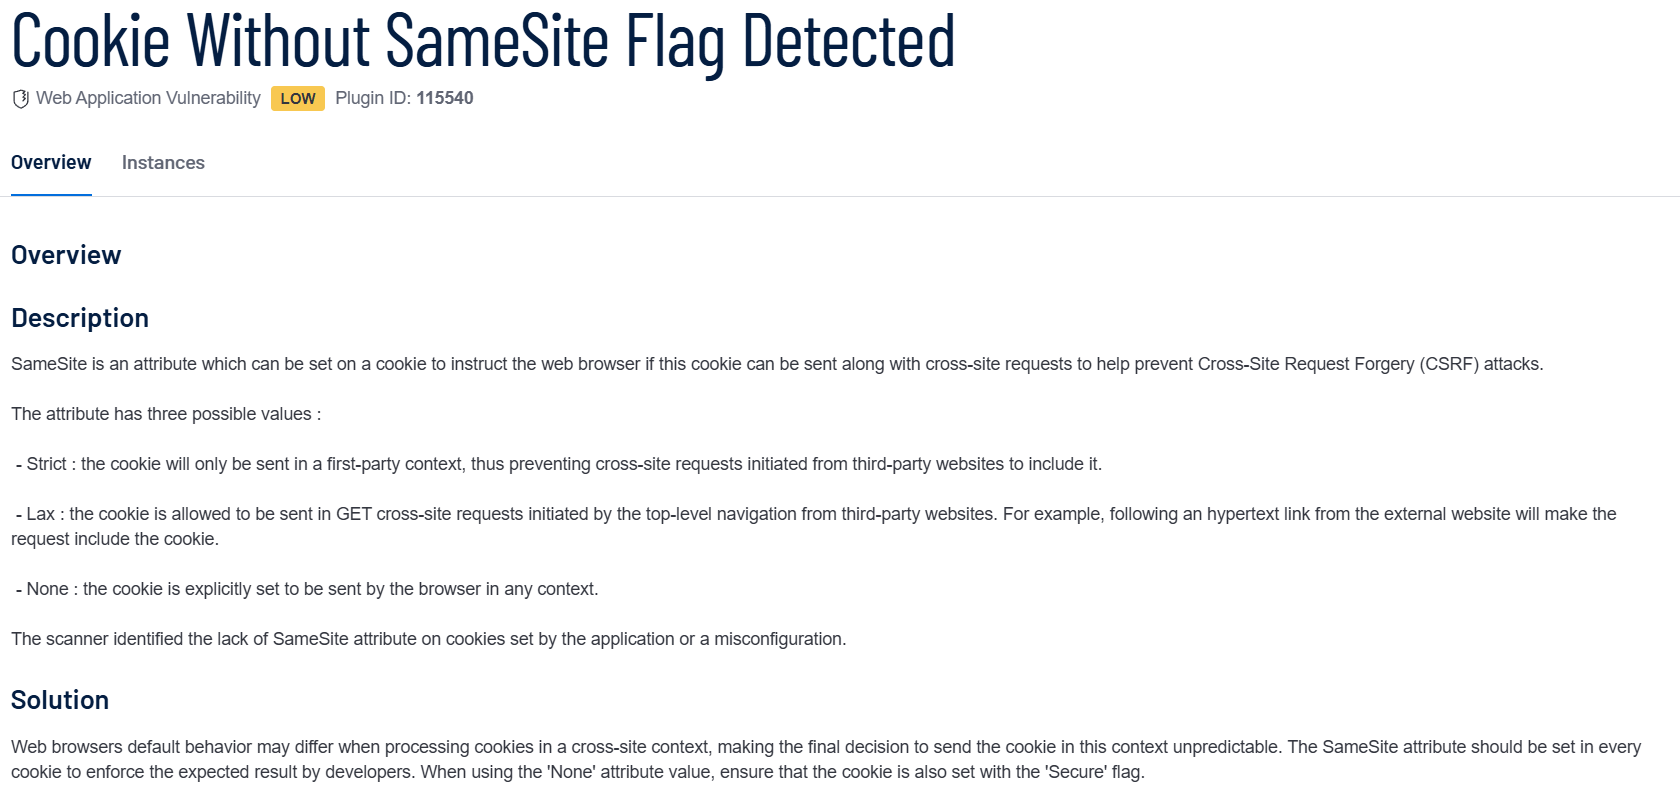
\includegraphics[width=0.8\textwidth]{assets/images-was/Vulnerabilidades em Cookies e Segurança de Sessão/Cookie Without SameSite Flag Detected.png}
                        \end{figure}
                        \FloatBarrier
                        \textbf{Descrição:} O atributo SameSite pode ser configurado em cookies para informar ao navegador se o cookie pode ser enviado junto com solicitações de sites diferentes (cross-site), ajudando a prevenir ataques de Cross-Site Request Forgery (CSRF). Esse atributo pode ter três valores possíveis:

    \begin{itemize}
    \item \textbf{Strict}: o cookie será enviado apenas em contextos de primeira parte, ou seja, apenas para o próprio site, impedindo que sites de terceiros o incluam em requisições.
    \item \textbf{Lax}: o cookie pode ser enviado em requisições GET de sites de terceiros, quando a navegação é iniciada pelo usuário em um link externo. Por exemplo, ao clicar em um link de um site externo, o cookie será incluído na solicitação.
    \item \textbf{None}: o cookie será explicitamente enviado pelo navegador em qualquer contexto, independentemente de ser uma requisição de primeira parte ou de terceiros.
    \end{itemize}

O scanner identificou que o aplicativo não configura ou configura incorretamente o atributo SameSite nos cookies. Isso pode resultar em um comportamento inesperado, já que o navegador pode, por padrão, enviar cookies em contextos cruzados, aumentando o risco de ataques CSRF.

\textbf{Solução:} Para mitigar essa vulnerabilidade, é essencial configurar o atributo SameSite em todos os cookies. O valor do atributo deve ser ajustado conforme o comportamento desejado. Ao usar o valor "None", é crucial também configurar o cookie com a flag \textit{Secure}, garantindo que ele seja enviado apenas por conexões HTTPS seguras.

\textbf{Total de URIs Afetadas:} None

\textbf{URIs Afetadas:}
\begin{itemize}
    \item \url{https://comunicacao.salvador.ba.gov.br}
    \item \url{https://www.credenciamento.salvador.ba.gov.br}
\end{itemize}

%-------------- FIM DA VULNERABILIDADE Cookie Without SameSite Flag Detected --------------
%-------------- INÍCIO DA VULNERABILIDADE Cookie Without Secure Flag Detected --------------
\item \textbf{\texttt{Cookie Without Secure Flag Detected}}

                        \begin{figure}[h!]
                        \centering
                        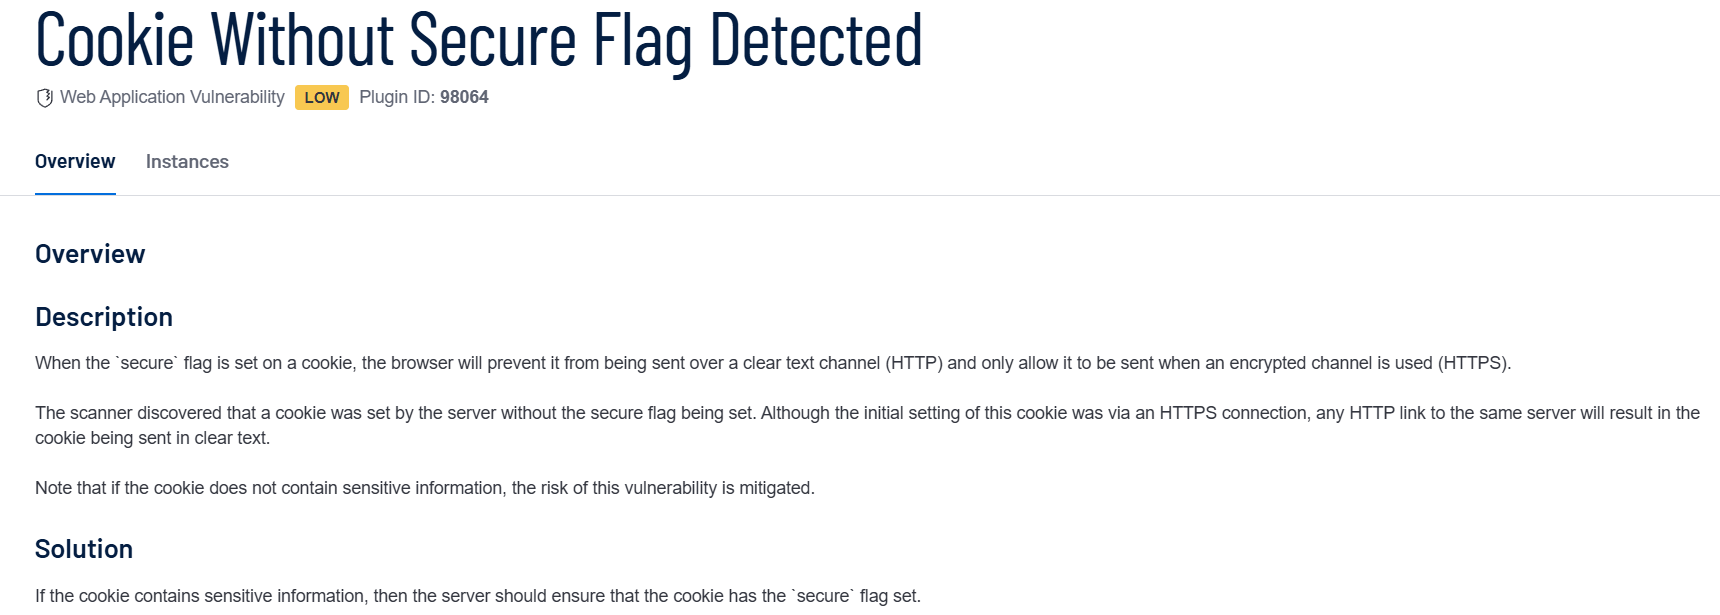
\includegraphics[width=0.8\textwidth]{assets/images-was/Vulnerabilidades em Cookies e Segurança de Sessão/Cookie Without Secure Flag Detected.png}
                        \end{figure}
                        \FloatBarrier
                        \textbf{Descrição:} Quando a flag secure é configurada em um cookie, o navegador impede que ele seja enviado através de um canal de texto claro (HTTP), permitindo que o cookie seja enviado apenas quando uma conexão segura (HTTPS) for utilizada. Isso ajuda a garantir que os cookies contendo informações sensíveis não sejam expostos em conexões não seguras.

O scanner detectou que o servidor configurou um cookie sem a flag secure. Embora o cookie tenha sido inicialmente configurado em uma conexão HTTPS, qualquer link HTTP para o mesmo servidor resultará no envio do cookie em texto claro, o que pode comprometer a segurança dos dados transmitidos, caso o cookie contenha informações sensíveis.

Vale ressaltar que, se o cookie não contiver informações sensíveis, o risco dessa vulnerabilidade é reduzido.

\textbf{Solução:} Se o cookie contiver informações sensíveis, como credenciais de usuário, dados financeiros ou informações pessoais, é essencial que o servidor configure o cookie com a flag secure. Isso garantirá que o cookie seja transmitido apenas em conexões HTTPS, protegendo assim a integridade e confidencialidade dos dados.

\textbf{Total de URIs Afetadas:} None

\textbf{URIs Afetadas:}
\begin{itemize}
    \item \url{https://comunicacao.salvador.ba.gov.br}
    \item \url{https://www.credenciamento.salvador.ba.gov.br}
\end{itemize}

%-------------- FIM DA VULNERABILIDADE Cookie Without Secure Flag Detected --------------
\end{enumerate}
%-------------- FIM DA SUBCATEGORIA Vulnerabilidades em Cookies e Segurança de Sessão --------------
%-------------- FIM DA CATEGORIA Vulnerabilidades em Cookies e Segurança de Sessão --------------
%-------------- INÍCIO DAS VULNERABILIDADES SEM CATEGORIA --------------
\section{Vulnerabilidades sem Categoria}
\begin{itemize}
    \item \texttt{Apache Tomcat 7.0.x < 7.0.99 Session Fixation}
    \item \texttt{Apache Tomcat 7.0.x < 7.0.107 Information Disclosure}
    \item \texttt{Apache Tomcat 7.0.x < 7.0.108 Multiple Vulnerabilities}
    \item \texttt{Apache Tomcat 7.0.0 < 7.0.85 Security Constraint Weakness}
    \item \texttt{Apache Tomcat 7.0.23 < 7.0.91 Open Redirect}
    \item \texttt{Apache Tomcat 7.0.x < 7.0.81 Multiple Vulnerabilities}
    \item \texttt{Apache Tomcat 7.0.x < 7.0.100 Multiple Vulnerabilities}
    \item \texttt{Apache Tomcat 7.0.x < 7.0.109 Authentication Weakness}
    \item \texttt{Apache Tomcat 7.0.x < 7.0.77 Information Disclosure}
    \item \texttt{Apache Tomcat 7.0.x < 7.0.104 Multiple Vulnerabilities}
    \item \texttt{Apache Tomcat 7.0.25 < 7.0.90 Multiple Vulnerabilities}
    \item \texttt{Apache Tomcat 7.0.0 < 7.0.94 Remote Code Execution on Windows}
    \item \texttt{Apache Tomcat 7.0.28 < 7.0.88 Denial of Service}
    \item \texttt{Apache Tomcat Unsupported Version}
    \item \texttt{Apache Tomcat 7.0.x < 7.0.78 Remote Error Page Manipulation}
    \item \texttt{CVS/SVN User Disclosure}
    \item \texttt{Apache Tomcat 7.0.x < 7.0.82 Remote Code Execution via JSP Upload}
    \item \texttt{Apache Tomcat 7.0.x < 7.0.99 Local Privilege Escalation}
    \item \texttt{Apache Tomcat 7.0.x < 7.0.105 Denial of Service}
    \item \texttt{Disclosed Hong Kong Identity Number}
    \item \texttt{DOM-based Cross-Site Scripting (XSS)}
    \item \texttt{Apache Tomcat Default Files}
    \item \texttt{Apache Tomcat Manager Detected}
\end{itemize}
%-------------- FIM DAS VULNERABILIDADES SEM CATEGORIA --------------

%-------------- FIM DA CATEGORIA Outras Vulnerabilidades Críticas e Explorações --------------
\section{Conclusão}

A auditoria de segurança cibernética realizada pela Gerência Especial de Segurança da Informação da COGEL revelou um cenário alarmante de vulnerabilidades e riscos no ambiente de aplicações e servidores da Prefeitura de Salvador, administrado pela  teste - teste. Foram identificadas diversas vulnerabilidades ativas, incluindo falhas críticas, altas, médias e baixas, que expõem o ambiente a possíveis ataques cibernéticos. Problemas graves, permissões incorretas de aplicações, suporte a protocolos e cifras criptográficas inseguras, e configurações inseguras em Sistemas Operacionais para aplicações críticas e a utilização de sistemas não suportados foram destacados.\\

A presença dessas vulnerabilidades representa uma ameaça significativa à segurança da informação e à continuidade dos serviços da Prefeitura de Salvador. A adoção de políticas de segurança mais rigorosas e a conformidade com normas como ISO/IEC 27001, NIST SP 800-53 e PCI DSS são essenciais para fortalecer a postura de segurança cibernética da instituição. A urgência na aplicação de patches e na implementação de medidas corretivas é imperativa para mitigar esses riscos e proteger a integridade, confidencialidade e disponibilidade dos serviços e dados da prefeitura e de seus cidadãos.\\

Por atingir seu objetivo, esta comissão encerra o presente instrumento ao tempo que declara o fim da Auditoria de Segurança Cibernética do Ambiente da teste - teste.

\newpage

\vspace*{\fill} % empurra o conteúdo para o final da página
\begin{flushright}
\textbf{Salvador, junho de 2025 \\%
Gerência Especial de Segurança da Informação \\%
Diretoria Técnica e de Infraestrutura \\%
Companhia de Governança Eletrônica do Salvador}
\end{flushright}

\end{document}
